% Options for packages loaded elsewhere
\PassOptionsToPackage{unicode}{hyperref}
\PassOptionsToPackage{hyphens}{url}
\PassOptionsToPackage{dvipsnames,svgnames,x11names}{xcolor}
%
\documentclass[
  letterpaper,
  DIV=11,
  numbers=noendperiod]{scrreprt}

\usepackage{amsmath,amssymb}
\usepackage{lmodern}
\usepackage{iftex}
\ifPDFTeX
  \usepackage[T1]{fontenc}
  \usepackage[utf8]{inputenc}
  \usepackage{textcomp} % provide euro and other symbols
\else % if luatex or xetex
  \usepackage{unicode-math}
  \defaultfontfeatures{Scale=MatchLowercase}
  \defaultfontfeatures[\rmfamily]{Ligatures=TeX,Scale=1}
\fi
% Use upquote if available, for straight quotes in verbatim environments
\IfFileExists{upquote.sty}{\usepackage{upquote}}{}
\IfFileExists{microtype.sty}{% use microtype if available
  \usepackage[]{microtype}
  \UseMicrotypeSet[protrusion]{basicmath} % disable protrusion for tt fonts
}{}
\makeatletter
\@ifundefined{KOMAClassName}{% if non-KOMA class
  \IfFileExists{parskip.sty}{%
    \usepackage{parskip}
  }{% else
    \setlength{\parindent}{0pt}
    \setlength{\parskip}{6pt plus 2pt minus 1pt}}
}{% if KOMA class
  \KOMAoptions{parskip=half}}
\makeatother
\usepackage{xcolor}
\setlength{\emergencystretch}{3em} % prevent overfull lines
\setcounter{secnumdepth}{5}
% Make \paragraph and \subparagraph free-standing
\ifx\paragraph\undefined\else
  \let\oldparagraph\paragraph
  \renewcommand{\paragraph}[1]{\oldparagraph{#1}\mbox{}}
\fi
\ifx\subparagraph\undefined\else
  \let\oldsubparagraph\subparagraph
  \renewcommand{\subparagraph}[1]{\oldsubparagraph{#1}\mbox{}}
\fi

\usepackage{color}
\usepackage{fancyvrb}
\newcommand{\VerbBar}{|}
\newcommand{\VERB}{\Verb[commandchars=\\\{\}]}
\DefineVerbatimEnvironment{Highlighting}{Verbatim}{commandchars=\\\{\}}
% Add ',fontsize=\small' for more characters per line
\usepackage{framed}
\definecolor{shadecolor}{RGB}{241,243,245}
\newenvironment{Shaded}{\begin{snugshade}}{\end{snugshade}}
\newcommand{\AlertTok}[1]{\textcolor[rgb]{0.68,0.00,0.00}{#1}}
\newcommand{\AnnotationTok}[1]{\textcolor[rgb]{0.37,0.37,0.37}{#1}}
\newcommand{\AttributeTok}[1]{\textcolor[rgb]{0.40,0.45,0.13}{#1}}
\newcommand{\BaseNTok}[1]{\textcolor[rgb]{0.68,0.00,0.00}{#1}}
\newcommand{\BuiltInTok}[1]{\textcolor[rgb]{0.00,0.23,0.31}{#1}}
\newcommand{\CharTok}[1]{\textcolor[rgb]{0.13,0.47,0.30}{#1}}
\newcommand{\CommentTok}[1]{\textcolor[rgb]{0.37,0.37,0.37}{#1}}
\newcommand{\CommentVarTok}[1]{\textcolor[rgb]{0.37,0.37,0.37}{\textit{#1}}}
\newcommand{\ConstantTok}[1]{\textcolor[rgb]{0.56,0.35,0.01}{#1}}
\newcommand{\ControlFlowTok}[1]{\textcolor[rgb]{0.00,0.23,0.31}{#1}}
\newcommand{\DataTypeTok}[1]{\textcolor[rgb]{0.68,0.00,0.00}{#1}}
\newcommand{\DecValTok}[1]{\textcolor[rgb]{0.68,0.00,0.00}{#1}}
\newcommand{\DocumentationTok}[1]{\textcolor[rgb]{0.37,0.37,0.37}{\textit{#1}}}
\newcommand{\ErrorTok}[1]{\textcolor[rgb]{0.68,0.00,0.00}{#1}}
\newcommand{\ExtensionTok}[1]{\textcolor[rgb]{0.00,0.23,0.31}{#1}}
\newcommand{\FloatTok}[1]{\textcolor[rgb]{0.68,0.00,0.00}{#1}}
\newcommand{\FunctionTok}[1]{\textcolor[rgb]{0.28,0.35,0.67}{#1}}
\newcommand{\ImportTok}[1]{\textcolor[rgb]{0.00,0.46,0.62}{#1}}
\newcommand{\InformationTok}[1]{\textcolor[rgb]{0.37,0.37,0.37}{#1}}
\newcommand{\KeywordTok}[1]{\textcolor[rgb]{0.00,0.23,0.31}{#1}}
\newcommand{\NormalTok}[1]{\textcolor[rgb]{0.00,0.23,0.31}{#1}}
\newcommand{\OperatorTok}[1]{\textcolor[rgb]{0.37,0.37,0.37}{#1}}
\newcommand{\OtherTok}[1]{\textcolor[rgb]{0.00,0.23,0.31}{#1}}
\newcommand{\PreprocessorTok}[1]{\textcolor[rgb]{0.68,0.00,0.00}{#1}}
\newcommand{\RegionMarkerTok}[1]{\textcolor[rgb]{0.00,0.23,0.31}{#1}}
\newcommand{\SpecialCharTok}[1]{\textcolor[rgb]{0.37,0.37,0.37}{#1}}
\newcommand{\SpecialStringTok}[1]{\textcolor[rgb]{0.13,0.47,0.30}{#1}}
\newcommand{\StringTok}[1]{\textcolor[rgb]{0.13,0.47,0.30}{#1}}
\newcommand{\VariableTok}[1]{\textcolor[rgb]{0.07,0.07,0.07}{#1}}
\newcommand{\VerbatimStringTok}[1]{\textcolor[rgb]{0.13,0.47,0.30}{#1}}
\newcommand{\WarningTok}[1]{\textcolor[rgb]{0.37,0.37,0.37}{\textit{#1}}}

\providecommand{\tightlist}{%
  \setlength{\itemsep}{0pt}\setlength{\parskip}{0pt}}\usepackage{longtable,booktabs,array}
\usepackage{calc} % for calculating minipage widths
% Correct order of tables after \paragraph or \subparagraph
\usepackage{etoolbox}
\makeatletter
\patchcmd\longtable{\par}{\if@noskipsec\mbox{}\fi\par}{}{}
\makeatother
% Allow footnotes in longtable head/foot
\IfFileExists{footnotehyper.sty}{\usepackage{footnotehyper}}{\usepackage{footnote}}
\makesavenoteenv{longtable}
\usepackage{graphicx}
\makeatletter
\def\maxwidth{\ifdim\Gin@nat@width>\linewidth\linewidth\else\Gin@nat@width\fi}
\def\maxheight{\ifdim\Gin@nat@height>\textheight\textheight\else\Gin@nat@height\fi}
\makeatother
% Scale images if necessary, so that they will not overflow the page
% margins by default, and it is still possible to overwrite the defaults
% using explicit options in \includegraphics[width, height, ...]{}
\setkeys{Gin}{width=\maxwidth,height=\maxheight,keepaspectratio}
% Set default figure placement to htbp
\makeatletter
\def\fps@figure{htbp}
\makeatother

\KOMAoption{captions}{tableheading}
\makeatletter
\makeatother
\makeatletter
\@ifpackageloaded{bookmark}{}{\usepackage{bookmark}}
\makeatother
\makeatletter
\@ifpackageloaded{caption}{}{\usepackage{caption}}
\AtBeginDocument{%
\ifdefined\contentsname
  \renewcommand*\contentsname{Table of contents}
\else
  \newcommand\contentsname{Table of contents}
\fi
\ifdefined\listfigurename
  \renewcommand*\listfigurename{List of Figures}
\else
  \newcommand\listfigurename{List of Figures}
\fi
\ifdefined\listtablename
  \renewcommand*\listtablename{List of Tables}
\else
  \newcommand\listtablename{List of Tables}
\fi
\ifdefined\figurename
  \renewcommand*\figurename{Figure}
\else
  \newcommand\figurename{Figure}
\fi
\ifdefined\tablename
  \renewcommand*\tablename{Table}
\else
  \newcommand\tablename{Table}
\fi
}
\@ifpackageloaded{float}{}{\usepackage{float}}
\floatstyle{ruled}
\@ifundefined{c@chapter}{\newfloat{codelisting}{h}{lop}}{\newfloat{codelisting}{h}{lop}[chapter]}
\floatname{codelisting}{Listing}
\newcommand*\listoflistings{\listof{codelisting}{List of Listings}}
\makeatother
\makeatletter
\@ifpackageloaded{caption}{}{\usepackage{caption}}
\@ifpackageloaded{subcaption}{}{\usepackage{subcaption}}
\makeatother
\makeatletter
\@ifpackageloaded{tcolorbox}{}{\usepackage[many]{tcolorbox}}
\makeatother
\makeatletter
\@ifundefined{shadecolor}{\definecolor{shadecolor}{rgb}{.97, .97, .97}}
\makeatother
\makeatletter
\makeatother
\ifLuaTeX
  \usepackage{selnolig}  % disable illegal ligatures
\fi
\IfFileExists{bookmark.sty}{\usepackage{bookmark}}{\usepackage{hyperref}}
\IfFileExists{xurl.sty}{\usepackage{xurl}}{} % add URL line breaks if available
\urlstyle{same} % disable monospaced font for URLs
\hypersetup{
  pdftitle={Modul Teknik Pengumpulan Data},
  pdfauthor={Muhammad Ammar Sahab},
  colorlinks=true,
  linkcolor={blue},
  filecolor={Maroon},
  citecolor={Blue},
  urlcolor={Blue},
  pdfcreator={LaTeX via pandoc}}

\title{Modul Teknik Pengumpulan Data}
\author{Muhammad Ammar Sahab}
\date{9/22/2022}

\begin{document}
\maketitle
\ifdefined\Shaded\renewenvironment{Shaded}{\begin{tcolorbox}[borderline west={3pt}{0pt}{shadecolor}, enhanced, frame hidden, interior hidden, boxrule=0pt, sharp corners, breakable]}{\end{tcolorbox}}\fi

\renewcommand*\contentsname{Table of contents}
{
\hypersetup{linkcolor=}
\setcounter{tocdepth}{2}
\tableofcontents
}
\bookmarksetup{startatroot}

\hypertarget{home}{%
\chapter*{Home}\label{home}}
\addcontentsline{toc}{chapter}{Home}

Modul Teknik Pengumpulan Data.

\bookmarksetup{startatroot}

\hypertarget{review-statistika-dasar}{%
\chapter{Review Statistika Dasar}\label{review-statistika-dasar}}

Mengumpulkan data pada dasarnya berarti mencari nilai-nilai dari
variabel tertentu yang menggambarkan suatu objek. \textbf{Skala
pengukuran} apa saja yang bisa dipakai? Dalam kata lain, jenis variabel
apa saja yang dapat menggambarkan objek?

\hypertarget{skala-nominal}{%
\subsection{Skala Nominal}\label{skala-nominal}}

Anggap Anda memiliki nilai data mengenai warna rambut dan mata sebagai
berikut:

\begin{longtable}[]{@{}lllr@{}}
\toprule()
Hair & Eye & Sex & n \\
\midrule()
\endhead
Black & Brown & Male & 32 \\
Brown & Brown & Male & 53 \\
Red & Brown & Male & 10 \\
Blond & Brown & Male & 3 \\
Black & Blue & Male & 11 \\
Brown & Blue & Male & 50 \\
Red & Blue & Male & 10 \\
Blond & Blue & Male & 30 \\
Black & Hazel & Male & 10 \\
Brown & Hazel & Male & 25 \\
Red & Hazel & Male & 7 \\
Blond & Hazel & Male & 5 \\
Black & Green & Male & 3 \\
Brown & Green & Male & 15 \\
Red & Green & Male & 7 \\
Blond & Green & Male & 8 \\
Black & Brown & Female & 36 \\
Brown & Brown & Female & 66 \\
Red & Brown & Female & 16 \\
Blond & Brown & Female & 4 \\
Black & Blue & Female & 9 \\
Brown & Blue & Female & 34 \\
Red & Blue & Female & 7 \\
Blond & Blue & Female & 64 \\
Black & Hazel & Female & 5 \\
Brown & Hazel & Female & 29 \\
Red & Hazel & Female & 7 \\
Blond & Hazel & Female & 5 \\
Black & Green & Female & 2 \\
Brown & Green & Female & 14 \\
Red & Green & Female & 7 \\
Blond & Green & Female & 8 \\
\bottomrule()
\end{longtable}

Skala tersebut disebut \textbf{skala nominal}. Skala nominal
\textbf{mengelompokkan} observasi, tanpa mengurutkan. Skala tersebut
berupa \textbf{kualitatif} sehingga tidak direpresentasikan angka. Dalam
kasus ini, tidak ada urutan tertentu; tidak ada warna mata terbaik, atau
warna rambut terbaik.

Contoh representasi skala nominal adalah \emph{factor} di bahasa R:

\begin{Shaded}
\begin{Highlighting}[numbers=left,,]
\FunctionTok{library}\NormalTok{(tidyverse)}
\end{Highlighting}
\end{Shaded}

\begin{verbatim}
-- Attaching packages --------------------------------------- tidyverse 1.3.2 --
v ggplot2 3.3.6     v purrr   0.3.4
v tibble  3.1.6     v dplyr   1.0.9
v tidyr   1.2.0     v stringr 1.4.0
v readr   2.1.2     v forcats 0.5.1
-- Conflicts ------------------------------------------ tidyverse_conflicts() --
x dplyr::filter() masks stats::filter()
x dplyr::lag()    masks stats::lag()
\end{verbatim}

\begin{Shaded}
\begin{Highlighting}[numbers=left,,]
\NormalTok{HairEyeColor }\SpecialCharTok{|\textgreater{}} 
\NormalTok{  tibble}\SpecialCharTok{::}\FunctionTok{as\_tibble}\NormalTok{() }\SpecialCharTok{|\textgreater{}} \FunctionTok{summary}\NormalTok{()}
\end{Highlighting}
\end{Shaded}

\begin{verbatim}
     Hair               Eye                Sex                  n        
 Length:32          Length:32          Length:32          Min.   : 2.00  
 Class :character   Class :character   Class :character   1st Qu.: 7.00  
 Mode  :character   Mode  :character   Mode  :character   Median :10.00  
                                                          Mean   :18.50  
                                                          3rd Qu.:29.25  
                                                          Max.   :66.00  
\end{verbatim}

Representasi data tersebut masih sebuah karakter. Ubah representasi
menjadi faktor:

\begin{Shaded}
\begin{Highlighting}[numbers=left,,]
\FunctionTok{library}\NormalTok{(tidyverse)}

\NormalTok{HairEyeColor }\SpecialCharTok{|\textgreater{}} 
\NormalTok{  tibble}\SpecialCharTok{::}\FunctionTok{as\_tibble}\NormalTok{() }\SpecialCharTok{|\textgreater{}}
  \FunctionTok{mutate\_if}\NormalTok{(is.character, as.factor) }\SpecialCharTok{|\textgreater{}}
  \FunctionTok{summary}\NormalTok{()}
\end{Highlighting}
\end{Shaded}

\begin{verbatim}
    Hair      Eye        Sex           n        
 Black:8   Blue :8   Female:16   Min.   : 2.00  
 Blond:8   Brown:8   Male  :16   1st Qu.: 7.00  
 Brown:8   Green:8               Median :10.00  
 Red  :8   Hazel:8               Mean   :18.50  
                                 3rd Qu.:29.25  
                                 Max.   :66.00  
\end{verbatim}

Setelah mengubah karakter menjadi representasi faktor, kita mengetahui
golongan-golongan rambut yang ada di dataset. Jika representasi skala
tertentu di suatu \emph{software} benar, \emph{software} tersebut sering
memiliki alat-alat untuk menanangani skala dengan baik.

\hypertarget{skala-ordinal}{%
\subsection{Skala Ordinal}\label{skala-ordinal}}

Jika kita memasukkan \emph{level} atau tingkatan dari faktor, dan
mengurutkannya, kita membuat suatu variabel dengan skala ordinal:

\begin{Shaded}
\begin{Highlighting}[]
\FunctionTok{factor}\NormalTok{(}\FunctionTok{c}\NormalTok{(}\StringTok{"SMA"}\NormalTok{, }\StringTok{"S1"}\NormalTok{, }\StringTok{"SMP"}\NormalTok{, }\StringTok{"SD"}\NormalTok{,}
         \StringTok{"SD"}\NormalTok{, }\StringTok{"S1"}\NormalTok{, }\StringTok{"S2"}\NormalTok{),}
       \AttributeTok{levels =} \FunctionTok{c}\NormalTok{(}\StringTok{"SD"}\NormalTok{, }\StringTok{"SMP"}\NormalTok{, }\StringTok{"SMA"}\NormalTok{, }\StringTok{"S1"}\NormalTok{, }\StringTok{"S2"}\NormalTok{)) }\SpecialCharTok{|\textgreater{}}
  \FunctionTok{ordered}\NormalTok{()}
\end{Highlighting}
\end{Shaded}

\begin{verbatim}
[1] SMA S1  SMP SD  SD  S1  S2 
Levels: SD < SMP < SMA < S1 < S2
\end{verbatim}

Objek ini disebut \emph{ordered factor}. Skala ordinal dapat diurutkan,
tetapi tidak dapat direpresentasikan dengan angka (masih
\textbf{kualitatif}).

\hypertarget{skala-interval}{%
\subsection{Skala Interval}\label{skala-interval}}

Kita mulai memasuki skala numerik. Artinya, variabel tersebut dapat
direpresentasikan \textbf{angka}, atau \textbf{kuantitatif}. Skala
interval memiliki jarak, tetapi tidak ada nol yang berarti. Skala
temperatur Celsius dan Fahrenheit tidak memiliki nol. Oleh karena itu,
tidak bisa diambil rasio. Atau, jarak antara 16 Agustus dan 17 Agustus
adalah satu hari, tapi tidak logis untuk mengatakan satu hari adalah
\(n\) kali hari lainnya.

\hypertarget{skala-rasio}{%
\subsection{Skala Rasio}\label{skala-rasio}}

Memiliki nol yang berarti, sehingga rasio dapat dibandingkan.
Jenis-jenis variabel ini termasuk tinggi, berat, lebar, dan lain-lain.

\hypertarget{exercise-skala-apa-saja}{%
\subsection{Exercise: Skala apa saja?}\label{exercise-skala-apa-saja}}

\begin{figure}

{\centering 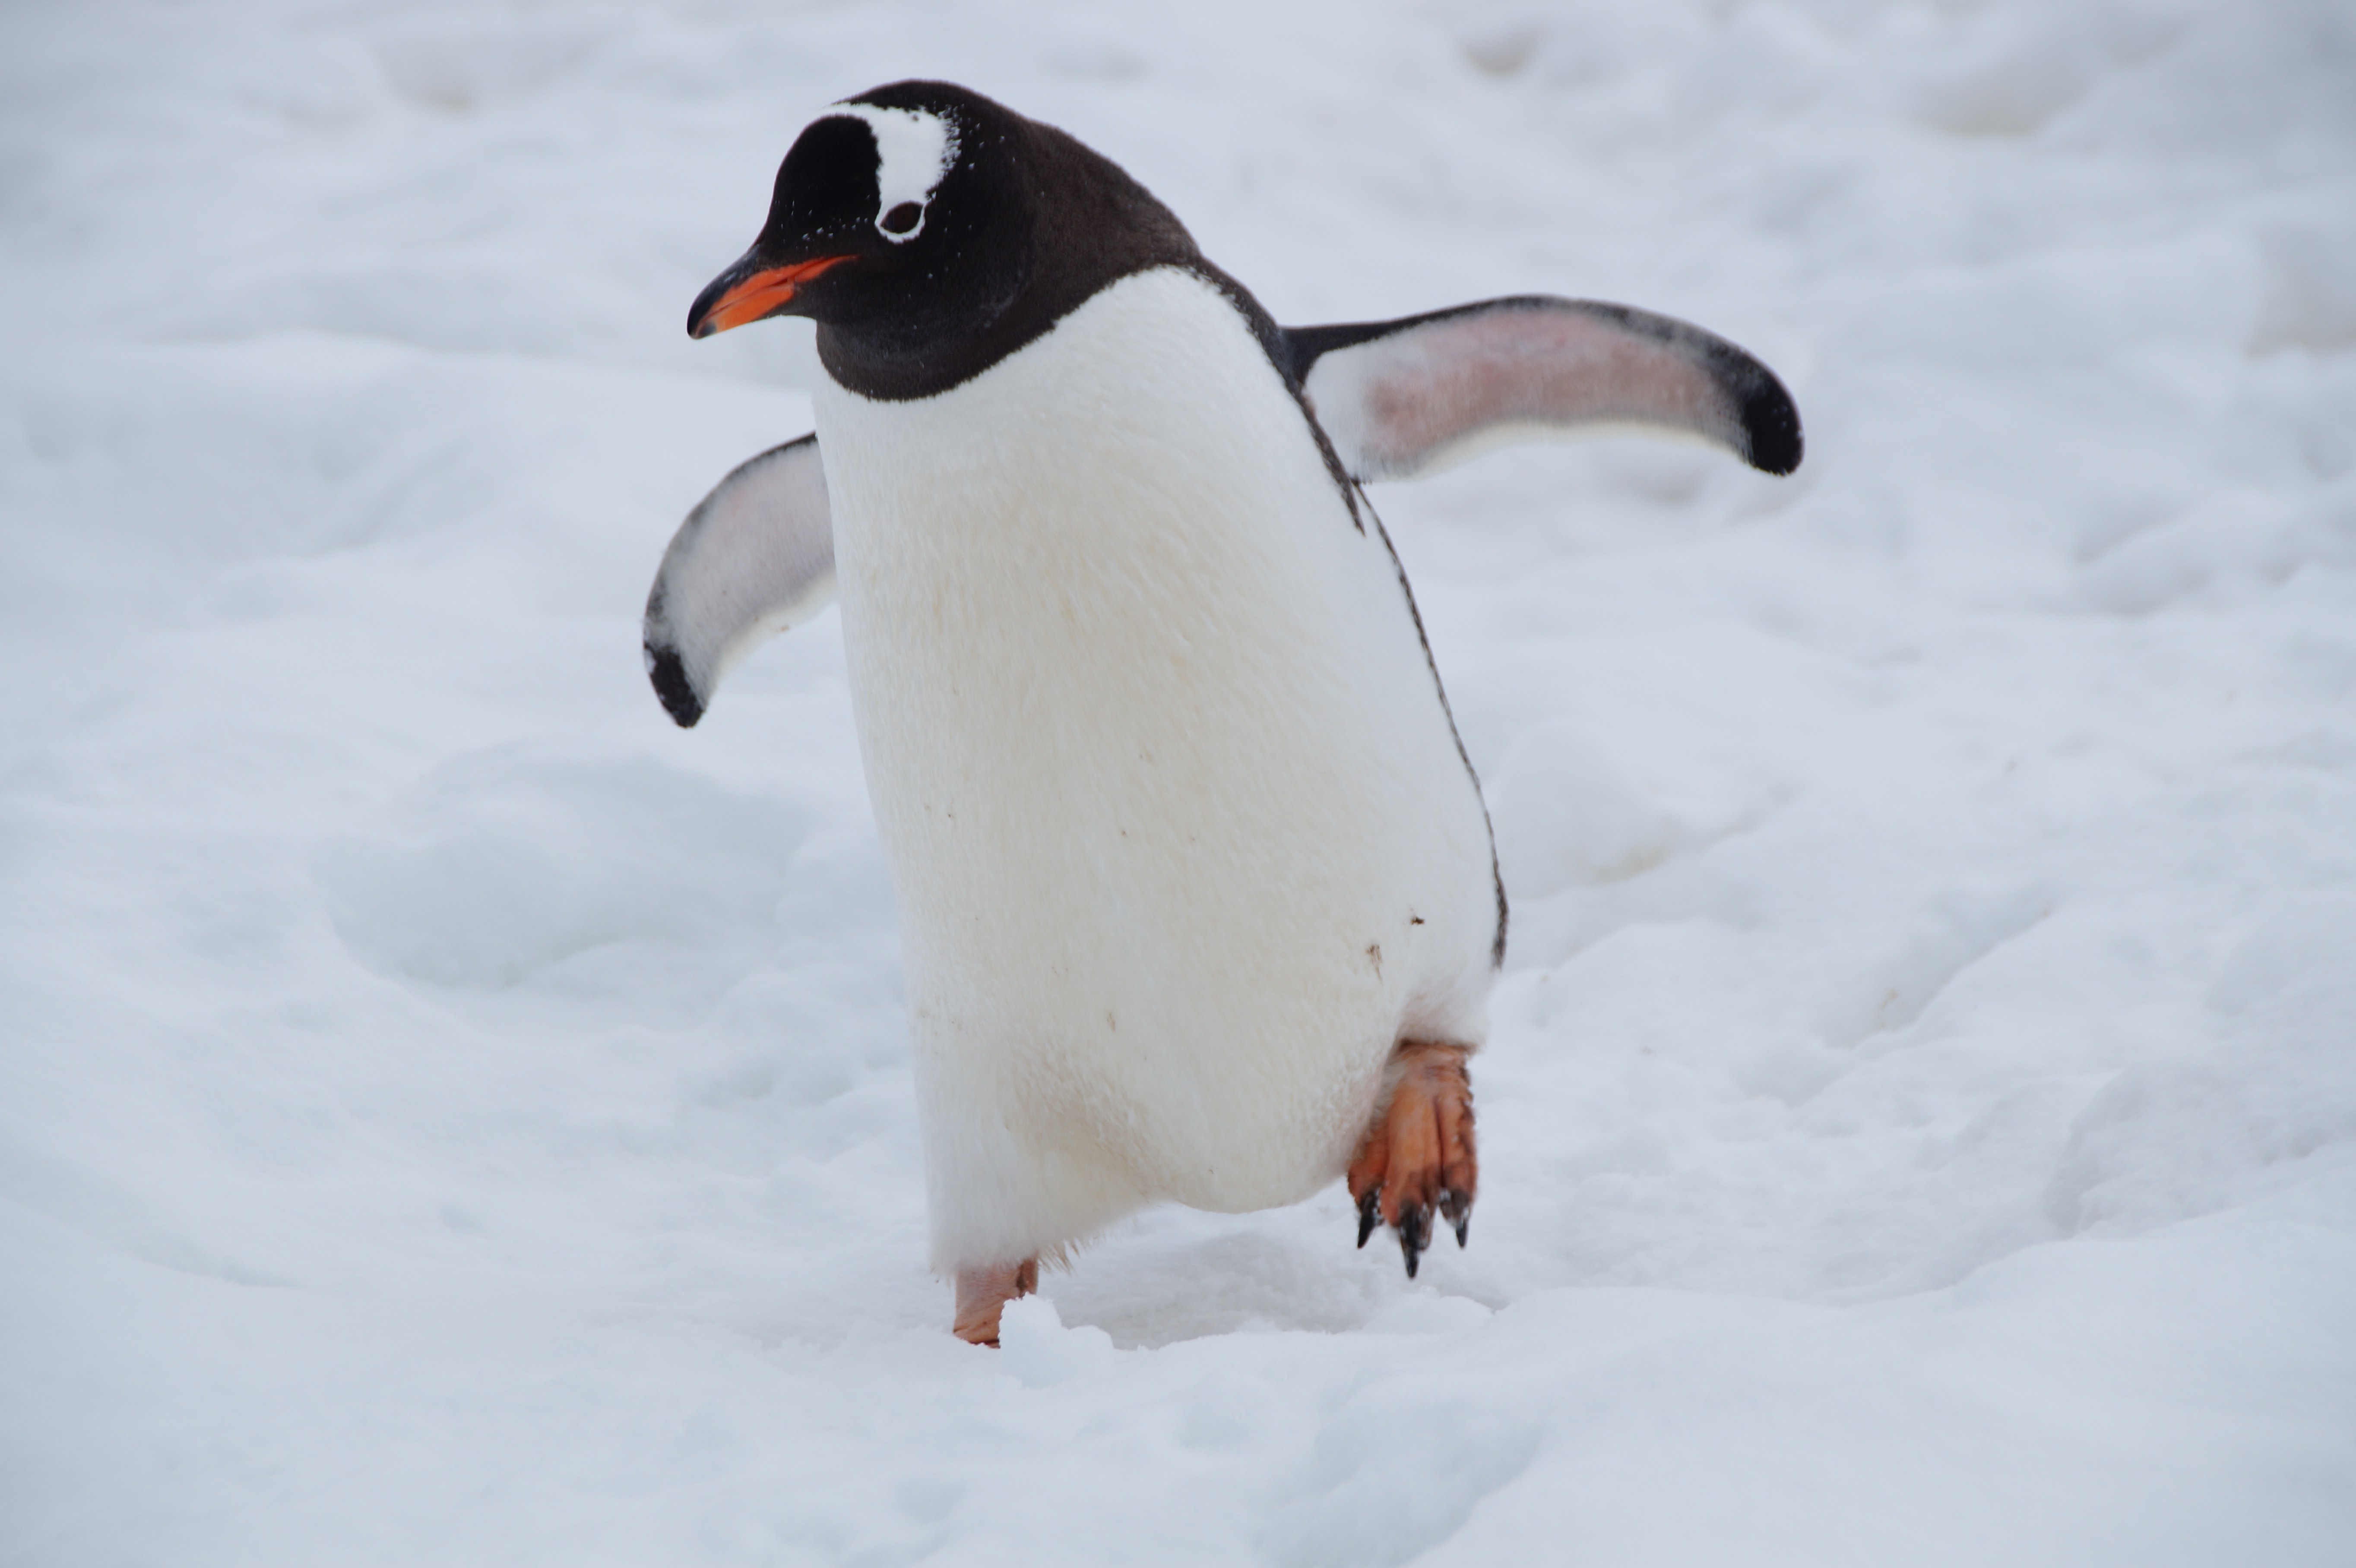
\includegraphics{./penguins2.jpg}

}

\caption{Penguins}

\end{figure}

\begin{verbatim}
      species          island    bill_length_mm  bill_depth_mm  
 Adelie   :152   Biscoe   :168   Min.   :32.10   Min.   :13.10  
 Chinstrap: 68   Dream    :124   1st Qu.:39.23   1st Qu.:15.60  
 Gentoo   :124   Torgersen: 52   Median :44.45   Median :17.30  
                                 Mean   :43.92   Mean   :17.15  
                                 3rd Qu.:48.50   3rd Qu.:18.70  
                                 Max.   :59.60   Max.   :21.50  
                                 NA's   :2       NA's   :2      
 flipper_length_mm  body_mass_g       sex           year     
 Min.   :172.0     Min.   :2700   female:165   Min.   :2007  
 1st Qu.:190.0     1st Qu.:3550   male  :168   1st Qu.:2007  
 Median :197.0     Median :4050   NA's  : 11   Median :2008  
 Mean   :200.9     Mean   :4202                Mean   :2008  
 3rd Qu.:213.0     3rd Qu.:4750                3rd Qu.:2009  
 Max.   :231.0     Max.   :6300                Max.   :2009  
 NA's   :2         NA's   :2                                 
\end{verbatim}

Tabel berasal dari dataset \textbf{Palmer Penguins}. Kalau tabel ini?

\begin{verbatim}
   agegp          alcgp         tobgp        ncases         ncontrols     
 25-34:15   0-39g/day:23   0-9g/day:24   Min.   : 0.000   Min.   : 0.000  
 35-44:15   40-79    :23   10-19   :24   1st Qu.: 0.000   1st Qu.: 1.000  
 45-54:16   80-119   :21   20-29   :20   Median : 1.000   Median : 4.000  
 55-64:16   120+     :21   30+     :20   Mean   : 2.273   Mean   : 8.807  
 65-74:15                                3rd Qu.: 4.000   3rd Qu.:10.000  
 75+  :11                                Max.   :17.000   Max.   :60.000  
\end{verbatim}

\begin{itemize}
\tightlist
\item
  agegp: Kelompok Usia
\item
  alcgp dan tobgp: Konsumsi alkohol dan tembakau
\item
  ncases dan ncontrols: Jumlah kasus dan kontrol untuk kanker esofagus.
\end{itemize}

\hypertarget{aplikasikan-mau-mencari-nilai-variabel-apa}{%
\subsection{Aplikasikan: Mau mencari nilai variabel
apa?}\label{aplikasikan-mau-mencari-nilai-variabel-apa}}

Misal kamu ingin tahu lebih lanjut tentang:

\begin{enumerate}
\def\labelenumi{\arabic{enumi}.}
\tightlist
\item
  Asisten,
\item
  Temanmu di kelas praktikum, dan
\item
  Gedung CCR.
\end{enumerate}

Apa variabel yang ingin kamu ketahui? Skala pengukurannya apa?

\hypertarget{populasi-dan-sampel}{%
\section{Populasi dan Sampel}\label{populasi-dan-sampel}}

Dalam tiap studi tersebut, asisten, teman kelas, dan gedung CCR
merupakan \textbf{populasi} - seperangkat objek dengan karakteristik
tertentu yang kita ingin ketahui. Kita mencari \textbf{parameter}
populasi - suatu kuantitas yang mendeskripsikan suatu aspek populasi.

\hypertarget{aplikasikan-tanya-asisten}{%
\subsection{Aplikasikan: tanya
asisten}\label{aplikasikan-tanya-asisten}}

Kamu punya 2 menit - kumpulkan data dari asisten!

Gunakan variabel-variabel yang kamu telah pikirkan di aplikasi
sebelumnya. Cari nilainya!

\hypertarget{aplikasikan-tanya-teman-kuliahmu}{%
\subsection{Aplikasikan: tanya teman
kuliahmu}\label{aplikasikan-tanya-teman-kuliahmu}}

Kamu punya 3 menit - kumpulkan data dari teman kuliahmu di ruang
praktikum!

Gunakan variabel-variabel yang kamu telah pikirkan di aplikasi
sebelumnya. Cari nilainya!

\hypertarget{sampling}{%
\section{Sampling}\label{sampling}}

Apakah kamu berhasil mengumpulkan data dari \textbf{semua} temanmu di
kelas ini? Bagaimana jika kamu ingin mengumpulkan data semua mahasiswa
IPB, semua warga Bogor, semua warga Indonesia? Terkadang, data populasi
\textbf{tidak bisa dikumpulkan}, atau \textbf{membutuhkan waktu dan
tenaga yang banyak}. Pencarian data juga dapat \textbf{destruktif} -
misal ingin mengetahui ketahanan baterai suatu merk jika dipanaskan -
tidak mungkin kita panaskan dan rusaki semua baterai yang diproduksi
merk tersebut!

\hypertarget{aplikasikan-cari-sampel}{%
\subsection{Aplikasikan: cari sampel}\label{aplikasikan-cari-sampel}}

Kamu memiliki waktu 2 menit. Sekarang tanyakan \emph{7} teman kamu saja!

Tiga orang akan maju dan deskripsikan hasilnya.

\hypertarget{statistik}{%
\subsection{Statistik}\label{statistik}}

Nilai yang ditemukan dari menanyakan 7 teman adalah \textbf{statistik}
sampel - suatu kuantitas yang mendeskripsikan suatu aspek sampel. Jika
kita menunjukkan grafik data, atau menunjukkan rataan/median, kita
melakukan \textbf{statistika deskriptif}. Namun, Apa yang kita bisa
katakan mengenai populasi, dengan data sampel?

Ambil satu variabel yang kamu cari datanya ke 7 teman kelas. Lalu
tanyakan ke semua teman; apakah berbeda?

\hypertarget{inferensia}{%
\subsection{Inferensia}\label{inferensia}}

Diperlukan \textbf{inferensia} untuk menduga parameter populasi dari
statistik sampel. Ilmu peluang digunakan untuk menduga dan menentukan
ketepatan dugaan tersebut.

\hypertarget{pengumpulan-data}{%
\section{Pengumpulan Data}\label{pengumpulan-data}}

Dari mana asal dataset \textbf{Palmer Penguins} dan \textbf{Esophageal
Cancer}? Pihak lain telah mengumpulkan datanya - ini disebut
\textbf{data sekunder}. Dalam mata kuliah ini, kita belajar mengumpulkan
data, seperti tadi - data yang dikumpulkan sendiri disebut \textbf{data
primer}.

Bagaimana kita mengumpulkan data untuk mendeskripsikan gedung CCR? Kita
telah melakukan \textbf{survei} - berinteraksi dengan objek sampel untuk
mengumpulkan data. Juga ada \textbf{sensus} - mengumpulkan data dari
seluruh populasi. Tentu kita tidak dapat menanyakan gedung CCR! Hanya
dapat \textbf{diobservasi} saja, tanpa interaksi.

Bagaimana jika datanya belum ada? Apa efek mendengarkan asisten sambil
jungkir balik pada nilai kuliah? Apakah ada yang kuliah sambil jungkir
balik? Harus dilakukan \textbf{percobaan} - memberikan perlakuan
tertentu, untuk membangkitkan data tersebut.

\hypertarget{exercise}{%
\section{Exercise}\label{exercise}}

https://openintro-ims.netlify.app/data-design.html\#chp2-exercises

Kerjakan no 1, 2, 7, 8.

\bookmarksetup{startatroot}

\hypertarget{konsep-dasar-survey-sampling}{%
\chapter{Konsep Dasar Survey
Sampling}\label{konsep-dasar-survey-sampling}}

Dalam \textbf{sensus}, peneliti mengamati seluruh anggota populasi.
Karena tenaga dan waktu yang dibutuhkan lama, sensus dilakukan dalam
jangka waktu panjang, misal 10 tahun sekali. Sedangkan, di
\textbf{survei} sebagian anggota populasi diamati.

\hypertarget{terminologi}{%
\section{Terminologi}\label{terminologi}}

\hypertarget{elemen}{%
\subsection{Elemen}\label{elemen}}

Proses penjelasan terminologi dimulai dari membayangkan pelaksanaan
survei. \textbf{Siapa yang ingin ada teliti}?

Objek apa yang Anda ingin ketahui karakteristiknya, atau Anda ingin
ukur?

Ini adalah elemen.

\begin{figure}[H]

{\centering \includegraphics[width=1.68167in,height=0.45833in]{./2-Terminologi_files/figure-latex/dot-figure-1.png}

}

\end{figure}

Grafik mengambarkan agregasi unit dari satu elemen ke kumpulan elemen.
\textbf{Populasi} adalah koleksi unsur yang ingin diduga
karakteristiknya. Sebagai contoh:

\begin{figure}[H]

{\centering \includegraphics[width=2.72292in,height=1.02083in]{./2-Terminologi_files/figure-latex/dot-figure-6.png}

}

\end{figure}

Warga Bogor adalah koleksi orang di Bogor. Kendaraan di Babakan Raya
adalah koleksi kendaraan.

\hypertarget{satuan-penarikan-contoh}{%
\subsection{Satuan penarikan contoh}\label{satuan-penarikan-contoh}}

Koleksi elemen dari populasi yang tidak \textbf{tumpang tindih} dan
mencakup seluruh populasi. Maksudnya? Paling sederhana \textbf{elemen =
satuan penarikan contoh}. Dalam contoh orang, tentu tidak mungkin
tumpang tindih. Apakah orang, jika digabung, mencakup seluruh warga
Bogor?

Namun, satuan penarikan contoh bisa juga tak sama dengan elemen:

\begin{figure}[H]

{\centering \includegraphics[width=3.04656in,height=0.45833in]{./2-Terminologi_files/figure-latex/dot-figure-5.png}

}

\end{figure}

Sama seperti diagram sebelumnya, panah menunjukkan arah dari unit yang
kecil ke unit yang besar. Elemen dapat digabung menjadi sebuah sampling
unit. Gabungan sampling unit menjadi populasi. Sebagai contoh:

\begin{figure}[H]

{\centering \includegraphics[width=3.7151in,height=1.02083in]{./2-Terminologi_files/figure-latex/dot-figure-4.png}

}

\end{figure}

Orang/mobil jika digabung dapat menjadi satu keluarga/satu mobil di
interval waktu tertentu. Jika sampling unit digabung, maka menjadi
populasi. Note: dalam contoh mobil, ada kemungkinan \textbf{tumpang
tindih}! Walaupun tiap orang hanya memiliki satu keluarga, bisa jadi
mobil yang di menit sebelumnya berada di Babakan Raya ada juga di menit
selanjutnya, karena macet!

\hypertarget{kerangka}{%
\subsection{Kerangka}\label{kerangka}}

Kerangka adalah \textbf{daftar} sampling unit di populasi. Ini dapat
digambarkan sebagai suatu tabel, di mana populasi dibagi menjadi
beberapa sampling unit. Lalu tiap sampling unit memiliki elemen:

\begin{figure}[H]

{\centering \includegraphics[width=2.9375in,height=3.10417in]{./2-Terminologi_files/figure-latex/dot-figure-3.png}

}

\end{figure}

Sebagai contoh:

\begin{figure}[H]

{\centering \includegraphics[width=3.04167in,height=2.70833in]{./2-Terminologi_files/figure-latex/dot-figure-2.png}

}

\end{figure}

Pemerintah Kota Bogor memiliki list Kepala Keluarga; lalu, di tiap KK
tersebut ada suatu keluarga yang beranggotakan elemen bernama Susi dan
Budi.

\hypertarget{sampel}{%
\subsection{Sampel}\label{sampel}}

Sampel adalah kumpulan satuan penarikan contoh dari kerangka. Misal,
ambil KK 1 dan 2. Hitung mobil di jam-jam tertentu

\hypertarget{exercise-1}{%
\subsection{Exercise}\label{exercise-1}}

\begin{enumerate}
\def\labelenumi{\arabic{enumi}.}
\tightlist
\item
  Cari suatu unit!
\item
  Kumpulan unit seperti apa yang kamu ingin duga karakteristiknya!
\item
  Kumpulan unit yang lebih kecil dari populasi apa saja yang mungkin
  terjadi?
\item
  Bagaimana bentuk kerangkanya?
\item
  Beri contoh pengambilan sampel dari kerangka tersebut.
\end{enumerate}

\hypertarget{sampling-1}{%
\section{Sampling}\label{sampling-1}}

\hypertarget{probability-sampling}{%
\subsection{Probability sampling}\label{probability-sampling}}

Dalam probability sampling, tiap anggota populasi memiliki probabilitas
untuk dipilih; probabilitasnya tidak perlu sama. Bisa saja:

\begin{enumerate}
\def\labelenumi{\arabic{enumi}.}
\tightlist
\item
  Probabilitas semua anggota dipilih sama.
\item
  Anggota kelompok tertentu, yang memang memiliki proporsi lebih besar
  di kerangka, memiliki probabilitas dipilih lebih besar.
\item
  Cara lain.
\end{enumerate}

\hypertarget{non-probability-sampling}{%
\subsection{Non-probability sampling}\label{non-probability-sampling}}

Probabilitas anggota populasi dipilih tidak diketahui di non-probability
sampling.

\hypertarget{sampling-error}{%
\subsection{Sampling error}\label{sampling-error}}

Berapa banyak dari kalian yang suka matematika?

Apa kesimpulan yang dapat diambil mengenai minat matematika mahasiswa
IPB? Kemungkinan susah untuk mengambil kesimpulan; mungkin saja
mahasiswa Statistika memiliki kemampuan matematika lebih tinggi, atau
ketertarikan matematika lebih tinggi. Mungkin saja mahasiswa Statistika
terlalu sering terekspos matematika sehingga tidak menyukai pelajaran
tersebut. Jika kita mengamati sebagian populasi (contoh), akan ada
keslahan karena contoh tersebut belum tentu mewakili keragaman populasi.
Jika mahasiswa dari berbagai jurusan diamati, kesimpulan lebih valid.
Lalu, dengan \textbf{probability sampling} tingkat kesalahan dapat
diduga.

\hypertarget{non-sampling-errors}{%
\section{Non-sampling errors}\label{non-sampling-errors}}

\hypertarget{nonobservation}{%
\subsection{Nonobservation}\label{nonobservation}}

Kesalahan yang terjadi karena gagal mengobservasi elemen:

\hypertarget{non-coverage}{%
\subsubsection{\texorpdfstring{\emph{Non-coverage}}{Non-coverage}}\label{non-coverage}}

Jika kerangka sampling tidak mencakup seluruh populasi, misal DPT tidak
lengkap atau tidak semua pengemudi punya SIM!

\hypertarget{non-response}{%
\subsubsection{\texorpdfstring{\emph{Non-response}}{Non-response}}\label{non-response}}

Error ini sering lebih fatal. Beberapa jenis error:

\begin{enumerate}
\def\labelenumi{\arabic{enumi}.}
\tightlist
\item
  Tidak bisa mengontak unit
\end{enumerate}

Tanpa keluar CCR, misal Anda coba survei jumlah pekerja dan pemasok
tempat makan kalian hari ini. Anda mungkin tak memiliki kontak elemen
survei tersebut! Namun, jika Anda menanyakan apa yang dimakan teman Anda
hari ini, hal tersebut mungkin ditemukan.

Misal, dengan contoh acak sederhana tiap elemen memiliki probabilitas
\(1/n\) untuk disampel. Apakah ada bisa menghitung probabilitas elemen
disampel jika sebenarnya dipilih elemen lain, elemen lain tidak ada,
lalu diganti elemen yang dekat? Ini susah.

Lalu, misal Anda melakukan survey ke rumah warga di jam siang. Ternyata,
orang berusia dewasa sedang kerja. Apa yang terjadi jika yang ditanya
adalah orang yang ada di rumah?

\begin{itemize}
\tightlist
\item
  Siapa yang mungkin di rumah warga pada jam siang?
\item
  Apakah mungkin profil orang tersebut beda dengan warga yang Anda cari?
\end{itemize}

\begin{enumerate}
\def\labelenumi{\arabic{enumi}.}
\setcounter{enumi}{1}
\tightlist
\item
  Unit tak bisa menjawab pertanyaan
\end{enumerate}

Buat pertanyaan yang susah dijawab orang. Bukan pertanyaan yang
sensitif, tetapi susah dimengerti/susah dicari jawabannya. Misal, apakah
Anda mengingat informasi:

\begin{enumerate}
\def\labelenumi{\arabic{enumi}.}
\tightlist
\item
  Pengeluaran dalam minggu ini.
\item
  Jarak berjalan kaki dalam hari ini.
\item
  Jumlah teman yang dikontak melalui WhatsApp dua hari ini.
\end{enumerate}

Belum tentu responden mengetahui/mengingat informasi yang kita ingin
tanyakan.

\begin{enumerate}
\def\labelenumi{\arabic{enumi}.}
\setcounter{enumi}{2}
\tightlist
\item
  Unit tidak ingin menjawab pertanyaan
\end{enumerate}

Ini cukup jelas.

\begin{enumerate}
\def\labelenumi{\arabic{enumi}.}
\setcounter{enumi}{3}
\tightlist
\item
  Dishonest interviewer
\end{enumerate}

Selain kesalahan dari responden, interviewer dapat tidak jujur dan
mengisi survei dengan sendirinya.

\hypertarget{errors-of-observation}{%
\subsection{Errors of observation}\label{errors-of-observation}}

Informasi dari elemen dapat diobservasi, tetapi diobservasi dengan
salah.

\hypertarget{interviewer-yang-tidak-netral}{%
\subsubsection{Interviewer yang tidak
netral}\label{interviewer-yang-tidak-netral}}

Apakah kalian suka cari masalah dengan orang? Jika interviewer dirasa
mendukung posisi tertentu, responden mungkin saja mencoba mengikuti
posisi interviewer, atau melawan posisi tersebut.

\hypertarget{kesalahan-responden}{%
\subsubsection{Kesalahan responden}\label{kesalahan-responden}}

\begin{enumerate}
\def\labelenumi{\arabic{enumi}.}
\tightlist
\item
  Jika Anda ditanya harga outfit Anda (dan kebetulan bagus outfitnya),
  apakah Anda ingin menaikkan harga outfit tersebut ke interviewer?
\item
  Jika Anda ditanya pernah melanggar aturan kampus, apakah Anda akan
  menjawab ya atau tidak?
\item
  Apakah Anda akan mengatakan jumlah uang bulanan Anda secara tepat jika
  ditanya?
\end{enumerate}

Inti dari aktivitas ini: responden memiliki motivasi yang berbeda-beda
untuk menjawab pertanyaan. Misal, responden ingin tampak mengikuti
aturan, ingin tampak kaya (atau menyembunyikan kekayaan), dan lain-lain.

\hypertarget{instrumen}{%
\subsubsection{Instrumen}\label{instrumen}}

Apa definisi Anda untuk:

\begin{enumerate}
\def\labelenumi{\arabic{enumi}.}
\tightlist
\item
  Anak
\item
  Pengangguran
\item
  Harga makanan murah
\end{enumerate}

Apakah definisi semua orang sama? Bagaimana jika survei menanyakan suatu
hal yang definisinya tidak jelas?

\hypertarget{input-data}{%
\subsubsection{Input Data}\label{input-data}}

Misal data sudah dikumpulkan. Apakah Anda pernah salah ketik? Apakah
komputer Anda pernah mengalami \emph{bug}? Data tersebut mungkin akan
berubah.

\hypertarget{mengurangi-kesalahan}{%
\section{Mengurangi kesalahan}\label{mengurangi-kesalahan}}

\hypertarget{trade-off-sampling-error-vs-non-sampling}{%
\subsection{Trade-off: sampling error vs
non-sampling}\label{trade-off-sampling-error-vs-non-sampling}}

Mana yang lebih mengikuti kaidah percontohan: mengambil contoh acak
mahasiswa IPB atau menanya teman? Siapa yang lebih mungkin merespon:
teman atau mahasiswa yang dicontoh acak?

Semakin besar ukuran sampel, semakin mendekati populasi. Kira-kira,
apakah Anda akan lebih lelah menanyakan lebih banyak orang lalu
memasukkan datanya? Jika lebih lelah, apakah Anda lebih mungkin salah?

\hypertarget{cara-mengurangi-non-sampling-error}{%
\subsection{Cara mengurangi non-sampling
error}\label{cara-mengurangi-non-sampling-error}}

\begin{enumerate}
\def\labelenumi{\arabic{enumi}.}
\tightlist
\item
  Callback
\end{enumerate}

Apakah chat Anda pernah tidak direspon? Apa yang Anda lakukan? Jika
di-chat lagi, apakah biasanya ada beberapa yang merespon kembali? Sama
saja, di survei, surveyor dapat kembali ke responden yang belum merespon
dan menanyakan pertanyaan yang sama lagi.

\begin{enumerate}
\def\labelenumi{\arabic{enumi}.}
\setcounter{enumi}{1}
\tightlist
\item
  Rewards
\end{enumerate}

Jika mengisi, dapat uang/dst. Pertanyaannya: apakah orang yang ingin
mengisi survei untuk dapat \emph{reward} beda dengan orang pada umumnya?
Mungkin orang tersebut memiliki keadaan finansial tertentu, atau lebih
suka uang.

\begin{enumerate}
\def\labelenumi{\arabic{enumi}.}
\setcounter{enumi}{2}
\tightlist
\item
  Melatih interviewer
\end{enumerate}

Interview dapat dilatih agar tampak netral dan mengetahui jawaban
jujur/tidak jujur

\begin{enumerate}
\def\labelenumi{\arabic{enumi}.}
\setcounter{enumi}{3}
\tightlist
\item
  Data checking
\end{enumerate}

Apakah mungkin:

\begin{itemize}
\tightlist
\item
  Seseorang berusia 1000 tahun?
\item
  Satu keluarga memiliki 50 anak?
\item
  Orang dewasa yang sudah menikah berusia 5 tahun?
\end{itemize}

Data-data tersebut perlu diperiksa.

\begin{enumerate}
\def\labelenumi{\arabic{enumi}.}
\setcounter{enumi}{4}
\tightlist
\item
  Memperbaiki kuesioner
\end{enumerate}

Beberapa aspek yang dapat diperhatikan:

\begin{itemize}
\tightlist
\item
  Urutan pertanyaan
\end{itemize}

Biasanya, responden ingin konsisten dengan jawabannya. Misal, ditanyakan
``Apakah Anda setuju dengan pemotongan subsidi BBM untuk peningkatan
dana pendidikan?''. Jika setelah pertanyaan itu ditanyakan ``Apakah Anda
setuju dengan pemotongan subsidi BBM?'', responden lebih mungkin
menjawab ``Ya''. Urutan tersebut pelru diperhatikan.

\begin{itemize}
\tightlist
\item
  Pertanyaan terbuka vs.~tertutup
\end{itemize}

Pertanyaaan terbuka memberi lebih banyak opsi bagi responden, tapi susah
diproses (non-sampling error meningkat). Pertanyaan tertutup dapat lebih
mudah diproses, tetapi harus dipastikan semua opsi yang hendak dipilih
responden ada.

\begin{itemize}
\tightlist
\item
  Opsi
\end{itemize}

Misal, opsi netral. Kebanyakan responden mungkin memilih opsi netral.
Apakah lebih baik untuk memaksa responden memilih?

\begin{itemize}
\tightlist
\item
  Wording
\end{itemize}

Responden mungkin tidak menyukai kata yang sangat negatif seperti
``melarang'', tetapi jika responden ditanya ``Apakah setuju dengan
membolehkan X'', bisa jadi banyak responden menjawab ``Tidak''.

\hypertarget{cara-pengumpulan-data}{%
\section{Cara pengumpulan data}\label{cara-pengumpulan-data}}

\hypertarget{personal-interview}{%
\subsection{Personal interview:}\label{personal-interview}}

\begin{itemize}
\tightlist
\item
  Apakah Anda akan merespon orang yang menanyakan Anda secara langsung?
\item
  Biasanya, Anda bicara mengikuti prosedur tertentu, atau mengikuti saja
  alur perbincangannya bagaimana?
\end{itemize}

Personal interview biasanya memiliki tingkat respon tinggi, tetapi bias
mungkin muncul dari interviewer.

\hypertarget{telephone-interview}{%
\subsection{Telephone interview}\label{telephone-interview}}

\begin{itemize}
\tightlist
\item
  Apakah semua kontak di HP Anda nomor orang? Apakah ada nomor bisnis?
  Nomor penipu? Nomor lama yang sudah tidak dipakai lagi? Mungkin saja
  kerangka percontohan tak akurat.
\item
  Biasanya, berapa lama Anda berbicara di telepon? Orang biasanya tak
  ingin berbicara lama.
\end{itemize}

\hypertarget{self-administered-questionnaire}{%
\subsection{Self-Administered
Questionnaire}\label{self-administered-questionnaire}}

\begin{itemize}
\tightlist
\item
  Tidak bisa memastikan responden mengisi atau tidak. Jika tidak ada
  yang mengingatkan/mengawasi, apakah Anda pernah lupa mengisi form?
\end{itemize}

Cara ingin sangat mudah, tetapi response rate rawan rendah.

\hypertarget{observasi}{%
\subsection{Observasi}\label{observasi}}

Misal Anda ingin meneliti berapa sering seseorang masuk kuliah. Apakah
Anda akan:

\begin{enumerate}
\def\labelenumi{\arabic{enumi}.}
\tightlist
\item
  Melihat absensi?
\item
  Menanyakan orang tersebut?
\end{enumerate}

Kadang, beberapa data lebih baik diobservasi langsung.

\hypertarget{tahapan-pembuatan-survey}{%
\section{Tahapan pembuatan survey}\label{tahapan-pembuatan-survey}}

Lakukan tahap 1-3!

\begin{enumerate}
\def\labelenumi{\arabic{enumi}.}
\tightlist
\item
  Tujuan survei apa?
\item
  Populasi target apa?
\item
  Dari mana Anda memperoleh sampling frame?
\end{enumerate}

Lalu lakukan tahap 5-7!

\begin{enumerate}
\def\labelenumi{\arabic{enumi}.}
\setcounter{enumi}{4}
\tightlist
\item
  Apakah Anda akan mewawancara responden?
\item
  Bagaimana cara Anda memastikan kuesioner reliabel dan valid?
\item
  Apakah pewawancara perlu dilatih; seperti apa?
\end{enumerate}

Terakhir, lakukan tahap 9-12!

\begin{enumerate}
\def\labelenumi{\arabic{enumi}.}
\setcounter{enumi}{8}
\tightlist
\item
  Bagaimana Anda mengumpulkan data dari responden?
\item
  Data ditaruh di mana?
\item
  Bagaimana Anda menganalisis data?
\item
  Bagaimana Anda melaporkan hasil survei?
\end{enumerate}

\bookmarksetup{startatroot}

\hypertarget{simple-random-sampling}{%
\chapter{Simple Random Sampling}\label{simple-random-sampling}}

Survei adalah \textbf{menduga} parameter populasi berdasarsarkan
informasi sampel. Faktor apa saja yang memengaruhi jumlah informasi di
sampel?

\begin{enumerate}
\def\labelenumi{\arabic{enumi}.}
\tightlist
\item
  Ukuran sampel
\item
  Keragaman di sampel - dapat dikontrol dengan rancangan percontohan
  yang baik. Paling sederhana: \textbf{simple random sampling}
\end{enumerate}

Dua poin penting:

\begin{enumerate}
\def\labelenumi{\arabic{enumi}.}
\tightlist
\item
  Semua elemen memiliki \textbf{peluang sama} untuk dipilih.
\item
  Pemilihan elemen \textbf{saling bebas}. Artinya, ada atau tidaknya
  elemen di sampel tidak memengaruhi probabilitas elemen lain dipilih.
\end{enumerate}

\hypertarget{exercise-apakah-ini-sampel-acak-sederhana}{%
\subsection{Exercise: apakah ini sampel acak
sederhana?}\label{exercise-apakah-ini-sampel-acak-sederhana}}

Do these methods produce a simple random sample of students from a class
of 30 students?

\begin{enumerate}
\def\labelenumi{\arabic{enumi}.}
\tightlist
\item
  Select the first six students on the class roll sheet
  (\emph{absensi}).
\item
  Pick a digit at random and select those students whose phone numbers
  end in that digit.
\item
  If the classroom has six rows of chairs with five seats in each row,
  choose a row at random and select all students in that row.
\item
  If the class consists of 15 boys and 15 girls, assign the boys the
  numbers from 1 to 15, and the girls the numbers from 16 to 30. Then
  use a random digit table to select six numbers from 1 to 30. Select
  the students assigned those numbers in your sample.
\item
  If the class consists of 15 boys and 15 girls, assign the boys the
  numbers from 1 to 15, and the girls the numbers from 16 to 30. Then
  use a random digit table to select three numbers from 1 to 15 and
  three numbers from 16 to 30. Select the students assigned those
  numbers in your sample.
\item
  Randomly choose a letter from the English alphabet and select for the
  sample those students whose last names begin with that letter. If no
  last name begins with that letter, randomly choose another letter from
  the alphabet.
\end{enumerate}

Kunci dari jawaban tersebut adalah:

\begin{enumerate}
\def\labelenumi{\arabic{enumi}.}
\tightlist
\item
  Select the first six students on the class roll sheet (\emph{absensi})
  - \textbf{peluang tak sama}. Enam orang pertama pasti terpilih, orang
  lainnya tidak mungkin terpilih.
\item
  Pick a digit at random and select those students whose phone numbers
  end in that digit - \textbf{sampel acak sederhana}. Alokasi nomor
  telpon cukup acak dan pemilihan juga acak.
\item
  If the classroom has six rows of chairs with five seats in each row,
  choose a row at random and select all students in that row -
  \textbf{tidak saling bebas}. Jika elemen di baris tersebut terpilih,
  pasti elemen lain juga terpilih. Lalu, elemen di baris lain pasti
  tidak terpilih.
\item
  If the class consists of 15 boys and 15 girls, assign the boys the
  numbers from 1 to 15, and the girls the numbers from 16 to 30. Then
  use a random digit table to select six numbers from 1 to 30. Select
  the students assigned those numbers in your sample - \textbf{sampel
  acak sederhana}.
\item
  If the class consists of 15 boys and 15 girls, assign the boys the
  numbers from 1 to 15, and the girls the numbers from 16 to 30. Then
  use a random digit table to select three numbers from 1 to 15 and
  three numbers from 16 to 30. Select the students assigned those
  numbers in your sample - \textbf{tidak saling bebas}. Jika 3 laki-laki
  dipilih, pasti tidak mungkin laki-laki lain dipilih.
\item
  Randomly choose a letter from the English alphabet and select for the
  sample those students whose last names begin with that letter. If no
  last name begins with that letter, randomly choose another letter from
  the alphabet. \textbf{Apakah nama-nama yang diawali alfabet tertentu
  lebih mungkin daripada alfabet lain?}. Selain itu, mungkin tidak
  saling bebas karena jika nama akhir yang banyak dimiliki orang
  terpilih; orang dengan nama lain tak mungkin terpilih.
\end{enumerate}

\hypertarget{contoh---rating-tv}{%
\subsection{Contoh - Rating TV}\label{contoh---rating-tv}}

\begin{itemize}
\tightlist
\item
  Apakah Anda memiliki acara televisi favorit?
\item
  Apakah acara favorit Anda pernah mengalami berhenti tayang
  (\emph{cancellation})?
\item
  Bagaimana stasiun televisi menentukan acara mana yang diberhentikan?
\end{itemize}

Nielsen Ratings - ambil 5000 rumah tangga di AS; tidak boleh ada
relawan. Dipasang meter elektronik yang mengetahui acara yang sedang
ditonton.

\hypertarget{cara-mengambil-sampel-acak-sederhana}{%
\subsection{Cara Mengambil Sampel Acak
Sederhana}\label{cara-mengambil-sampel-acak-sederhana}}

Cara salah:

\begin{itemize}
\tightlist
\item
  Haphazard: sesuai keinginan peneliti
\item
  Representative: ambil sampel yang dianggap mewakili populasi
\end{itemize}

Peneliti bisa saja berbias dan walaupun representatif, \textbf{tingkat
kesalahan tak dapat diketahui} karena tidak diketahui struktur
probabilitasnya.

Cara benar:

\begin{itemize}
\tightlist
\item
  Undian - masukkan angka 1 sampai n, ambil!
\item
  Tabel angka acak - biasananya menggunakan komputer!
\end{itemize}

\hypertarget{exercise-deskripsikan-bias}{%
\subsection{Exercise: deskripsikan
bias}\label{exercise-deskripsikan-bias}}

\begin{enumerate}
\def\labelenumi{\arabic{enumi}.}
\tightlist
\item
  A student wants to determine the average size of farms in a county in
  Iowa. He drops some rice randomly on a map of the county and uses the
  farms hit by grains of rice as the sample (\emph{county - kabupaten}).
\item
  To find the average length of string in a bag, a student reaches in,
  mixes up the strings, selects one, mixes them up again, selects
  another, and so on (\emph{string - tali}).
\item
  To estimate the percentage of students who passed the first Advanced
  Placement Statistics exam, a teacher on an Internet discussion list
  for teachers of AP Statistics asked teachers on the list to report to
  him how many of their students took the test and how many passed
  (\emph{discussion list - forum diskusi}).
\item
  In 1984, Ann Landers conducted a poll on the marital happiness of
  women by asking women to write to her (\emph{marital - pernikahan}).
\item
  In a study about whether valedictorians ``succeed big in life,'' a
  professor ``traveled across Illinois, attending high school
  graduations and selecting 81 students to participate. . . . He picked
  students from the most diverse communities possible, from little rural
  schools to rich suburban schools near Chicago to city schools.''
\end{enumerate}

\emph{Valedictorian: lulusan terbaik.}

Jawaban dari exercise tersebut adalah:

\begin{enumerate}
\def\labelenumi{\arabic{enumi}.}
\tightlist
\item
  A student wants to determine the average size of farms in a county in
  Iowa. He drops some rice randomly on a map of the county and uses the
  farms hit by grains of rice as the sample (\emph{county - kabupaten})
  - \textbf{proses ini cukup acak}.
\item
  To find the average length of string in a bag, a student reaches in,
  mixes up the strings, selects one, mixes them up again, selects
  another, and so on (\emph{string - tali}) - \textbf{proses ini juga
  cukup acak}.
\item
  To estimate the percentage of students who passed the first Advanced
  Placement Statistics exam, a teacher on an Internet discussion list
  for teachers of AP Statistics asked teachers on the list to report to
  him how many of their students took the test and how many passed
  (\emph{discussion list - forum diskusi}) - \textbf{ada bias yang
  muncul karena guru-guru yang menjawab di forum diskusi belum tentu
  representatif terhadap guru umumnya}. Mungkin, guru tersebut lebih
  ambisius.
\item
  In 1984, Ann Landers conducted a poll on the marital happiness of
  women by asking women to write to her (\emph{marital - pernikahan}).
  \textbf{Bias yang sama}. Orang yang menulis tentang pernikahannya
  mungkin memiliki perasaan ekstrim, seperti sangat senang atau sangat
  marah.
\item
  In a study about whether valedictorians ``succeed big in life,'' a
  professor ``traveled across Illinois, attending high school
  graduations and selecting 81 students to participate. . . . He picked
  students from the most diverse communities possible, from little rural
  schools to rich suburban schools near Chicago to city schools.''
\end{enumerate}

\textbf{Walaupun representatif, tingkat kesalahan tak dapat
diperkirakan}.

Untuk melakukan pengacakan, sering dipakai \emph{random number
generator}:

\hypertarget{excel}{%
\subsubsection{Excel}\label{excel}}

Gunakan fungsi \texttt{=RAND()}: 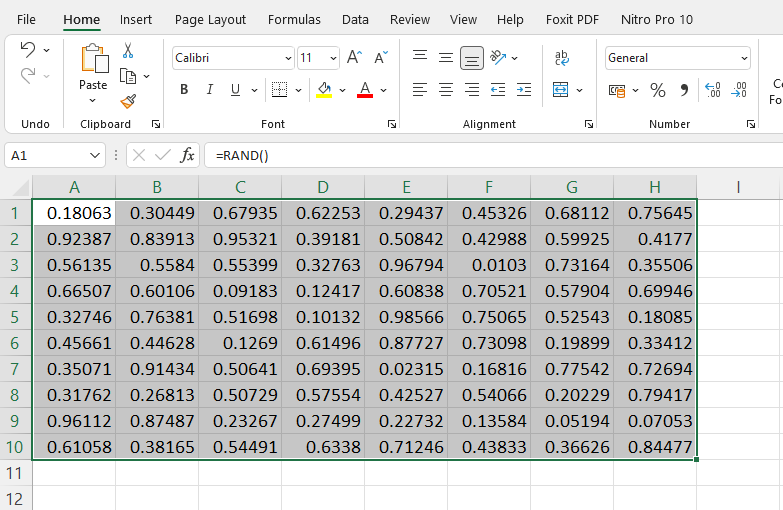
\includegraphics{./excel-rand.png}

\hypertarget{r}{%
\subsubsection{R}\label{r}}

Gunakan fungsi \texttt{runif()}:

\begin{Shaded}
\begin{Highlighting}[]
\FunctionTok{runif}\NormalTok{(}\DecValTok{100}\NormalTok{) }\SpecialCharTok{|\textgreater{}} \FunctionTok{head}\NormalTok{(}\DecValTok{5}\NormalTok{)}
\end{Highlighting}
\end{Shaded}

\begin{verbatim}
[1] 0.8521342 0.5460658 0.9064181 0.4989673 0.6854146
\end{verbatim}

\hypertarget{python}{%
\subsubsection{Python}\label{python}}

Gunakan rng dari package \texttt{numpy}:

\begin{Shaded}
\begin{Highlighting}[]
\ImportTok{import}\NormalTok{ numpy }\ImportTok{as}\NormalTok{ np}

\NormalTok{rng }\OperatorTok{=}\NormalTok{ np.random.default\_rng(}\DecValTok{3854}\NormalTok{)}
\NormalTok{rng.random(}\DecValTok{5}\NormalTok{)}
\end{Highlighting}
\end{Shaded}

\begin{verbatim}
array([0.50955422, 0.53163209, 0.98811285, 0.47079458, 0.08600762])
\end{verbatim}

\hypertarget{memilih-sampel-acak-sederhana}{%
\section{Memilih sampel acak
sederhana}\label{memilih-sampel-acak-sederhana}}

Algoritma:

\begin{enumerate}
\def\labelenumi{\arabic{enumi}.}
\tightlist
\item
  Buat angka acak sejumlah elemen yang ada
\item
  Pasangkan tiap elemen dengan angka acak
\item
  Urutkan elemen sesuai angka acak, pilih n teratas.
\end{enumerate}

\hypertarget{step-0-lihat-dataset-dan-jumlah-row}{%
\subsection{Step 0: Lihat Dataset dan Jumlah
Row}\label{step-0-lihat-dataset-dan-jumlah-row}}

Sebelum melaksanakan algoritma tersebut, lihat dataset dan jumlah row:

\hypertarget{excel-1}{%
\subsubsection{Excel}\label{excel-1}}

Pertama, ambil data dari csv:

\begin{figure}

{\centering 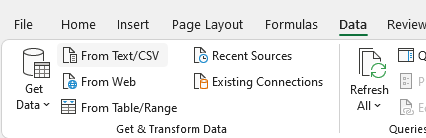
\includegraphics{./step0-getdata.png}

}

\caption{Pengambilan data}

\end{figure}

Pilih file, lalu preview dan load:

\begin{figure}

{\centering 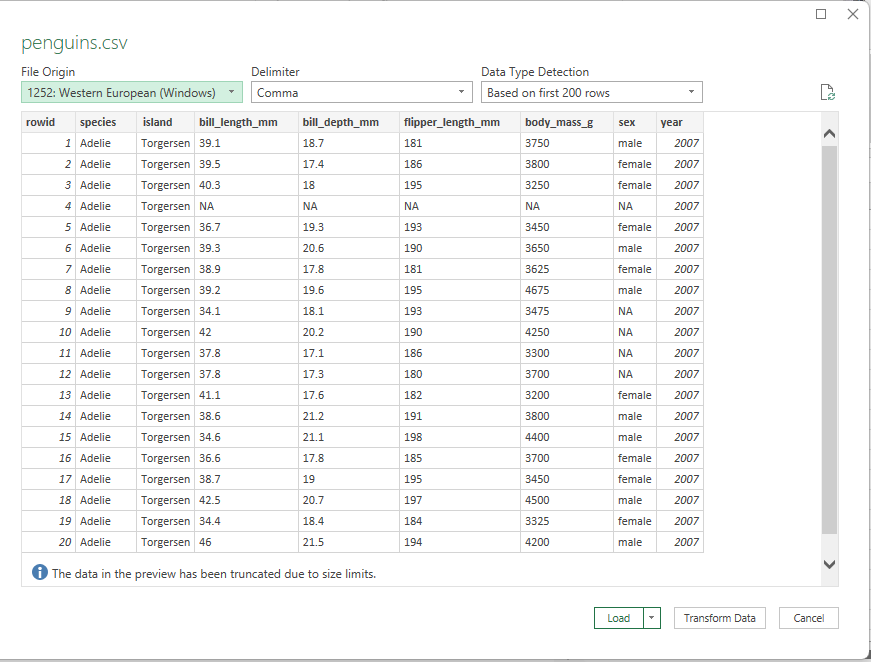
\includegraphics{./step0-preview.png}

}

\caption{Preview}

\end{figure}

Data akan terlihat di Excel.

\hypertarget{r-1}{%
\subsubsection{R}\label{r-1}}

Langkah relatif sama. Baca CSV, lihat file.

\begin{Shaded}
\begin{Highlighting}[]
\NormalTok{penguins }\OtherTok{\textless{}{-}} \FunctionTok{read.csv}\NormalTok{(}\StringTok{"penguins.csv"}\NormalTok{)}

\NormalTok{penguins }\SpecialCharTok{|\textgreater{}} \FunctionTok{head}\NormalTok{(}\DecValTok{3}\NormalTok{)}
\end{Highlighting}
\end{Shaded}

\begin{verbatim}
  rowid species    island bill_length_mm bill_depth_mm flipper_length_mm
1     1  Adelie Torgersen           39.1          18.7               181
2     2  Adelie Torgersen           39.5          17.4               186
3     3  Adelie Torgersen           40.3          18.0               195
  body_mass_g    sex year
1        3750   male 2007
2        3800 female 2007
3        3250 female 2007
\end{verbatim}

\begin{Shaded}
\begin{Highlighting}[]
\NormalTok{penguins }\SpecialCharTok{|\textgreater{}} \FunctionTok{nrow}\NormalTok{()}
\end{Highlighting}
\end{Shaded}

\begin{verbatim}
[1] 344
\end{verbatim}

\hypertarget{python-1}{%
\subsubsection{Python}\label{python-1}}

\begin{Shaded}
\begin{Highlighting}[]
\ImportTok{import}\NormalTok{ pandas }\ImportTok{as}\NormalTok{ pd}

\NormalTok{penguins }\OperatorTok{=}\NormalTok{ pd.read\_csv(}\StringTok{"penguins.csv"}\NormalTok{)}
\BuiltInTok{print}\NormalTok{(penguins.head())}
\end{Highlighting}
\end{Shaded}

\begin{verbatim}
   rowid species     island  ...  body_mass_g     sex  year
0      1  Adelie  Torgersen  ...       3750.0    male  2007
1      2  Adelie  Torgersen  ...       3800.0  female  2007
2      3  Adelie  Torgersen  ...       3250.0  female  2007
3      4  Adelie  Torgersen  ...          NaN     NaN  2007
4      5  Adelie  Torgersen  ...       3450.0  female  2007

[5 rows x 9 columns]
\end{verbatim}

\begin{Shaded}
\begin{Highlighting}[]
\BuiltInTok{print}\NormalTok{(}\BuiltInTok{len}\NormalTok{(penguins.index))}
\end{Highlighting}
\end{Shaded}

\begin{verbatim}
344
\end{verbatim}

\hypertarget{step-1-2-angka-acak-pasangkan}{%
\subsection{Step 1-2: Angka Acak,
Pasangkan}\label{step-1-2-angka-acak-pasangkan}}

Lalu, buat angka acak. Angka acak ini merupakan kolom baru di dataset.
Tiap elemen mendapat angka acak yang unik. Bagaimana kita tahu jumlah
angka acak yang perlu dibuat? Cari terlebih dahulu jumlah elemen di
dataset.

\hypertarget{excel-2}{%
\subsubsection{Excel}\label{excel-2}}

Buat angka acak dengan \texttt{rand()}.

\begin{figure}

{\centering 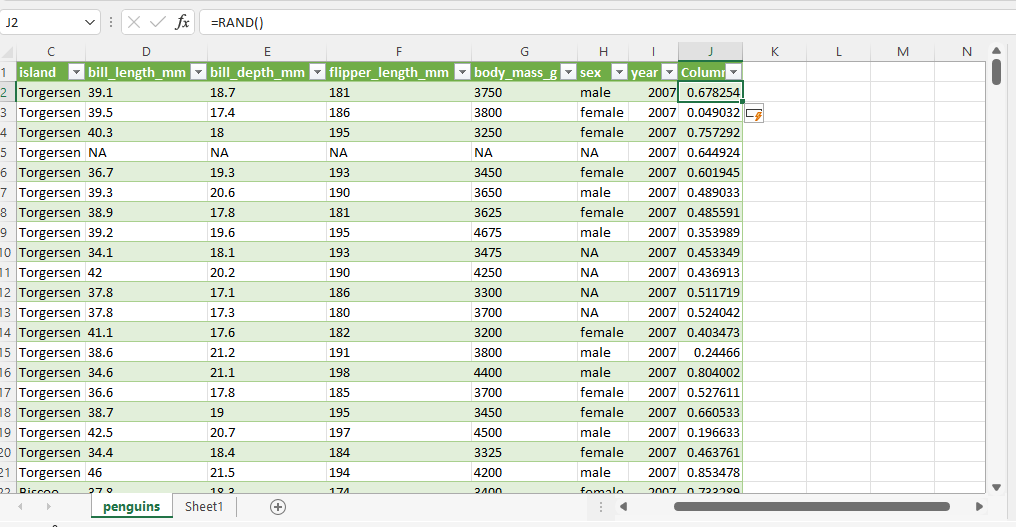
\includegraphics{./step1-genrand.png}

}

\caption{Angka acak}

\end{figure}

Namun, angka acak ini akan selalu berubah jika di-\emph{sort}. Oleh
karena itu, \emph{copy}, (\textbf{CTRL+C}) lalu paste \emph{as value}.
Opsi \emph{paste as value} ditemukan dengan meng-klik kanan:

\begin{figure}

{\centering 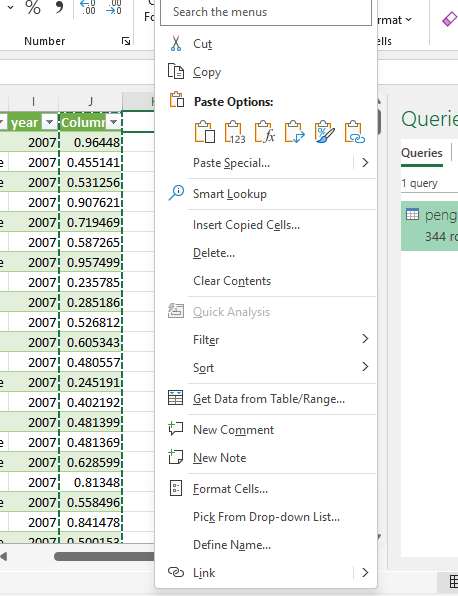
\includegraphics{./step1-paste1.png}

}

\caption{Menu paste}

\end{figure}

Lalu ditemukan opsi tersebut; opsi berupa suatu \emph{clipboard} (kertas
di atas papan jalan) dengan angka 123:

\begin{figure}

{\centering 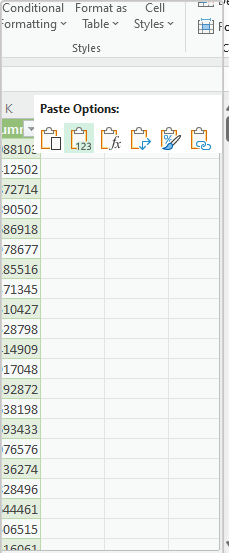
\includegraphics{./step1-paste2.png}

}

\caption{Paste as value}

\end{figure}

\hypertarget{r-2}{%
\subsubsection{R}\label{r-2}}

Jumlah angka acak dicari menggunakan nrow dari dataset. Mutate
menghasilkan peubah baru.

\begin{Shaded}
\begin{Highlighting}[]
\FunctionTok{library}\NormalTok{(dplyr)}
\end{Highlighting}
\end{Shaded}

\begin{verbatim}

Attaching package: 'dplyr'
\end{verbatim}

\begin{verbatim}
The following objects are masked from 'package:stats':

    filter, lag
\end{verbatim}

\begin{verbatim}
The following objects are masked from 'package:base':

    intersect, setdiff, setequal, union
\end{verbatim}

\begin{Shaded}
\begin{Highlighting}[]
\NormalTok{penguins }\OtherTok{\textless{}{-}} \FunctionTok{read.csv}\NormalTok{(}\StringTok{"penguins.csv"}\NormalTok{)}
\NormalTok{penguins }\OtherTok{\textless{}{-}}\NormalTok{ penguins }\SpecialCharTok{|\textgreater{}} \FunctionTok{mutate}\NormalTok{(}\AttributeTok{rando =} \FunctionTok{runif}\NormalTok{(}\FunctionTok{nrow}\NormalTok{(penguins)))}

\NormalTok{penguins }\SpecialCharTok{|\textgreater{}} \FunctionTok{head}\NormalTok{(}\DecValTok{3}\NormalTok{) }\SpecialCharTok{|\textgreater{}}\NormalTok{ knitr}\SpecialCharTok{::}\FunctionTok{kable}\NormalTok{()}
\end{Highlighting}
\end{Shaded}

\begin{longtable}[]{@{}
  >{\raggedleft\arraybackslash}p{(\columnwidth - 18\tabcolsep) * \real{0.0571}}
  >{\raggedright\arraybackslash}p{(\columnwidth - 18\tabcolsep) * \real{0.0762}}
  >{\raggedright\arraybackslash}p{(\columnwidth - 18\tabcolsep) * \real{0.0952}}
  >{\raggedleft\arraybackslash}p{(\columnwidth - 18\tabcolsep) * \real{0.1429}}
  >{\raggedleft\arraybackslash}p{(\columnwidth - 18\tabcolsep) * \real{0.1333}}
  >{\raggedleft\arraybackslash}p{(\columnwidth - 18\tabcolsep) * \real{0.1714}}
  >{\raggedleft\arraybackslash}p{(\columnwidth - 18\tabcolsep) * \real{0.1143}}
  >{\raggedright\arraybackslash}p{(\columnwidth - 18\tabcolsep) * \real{0.0667}}
  >{\raggedleft\arraybackslash}p{(\columnwidth - 18\tabcolsep) * \real{0.0476}}
  >{\raggedleft\arraybackslash}p{(\columnwidth - 18\tabcolsep) * \real{0.0952}}@{}}
\toprule()
\begin{minipage}[b]{\linewidth}\raggedleft
rowid
\end{minipage} & \begin{minipage}[b]{\linewidth}\raggedright
species
\end{minipage} & \begin{minipage}[b]{\linewidth}\raggedright
island
\end{minipage} & \begin{minipage}[b]{\linewidth}\raggedleft
bill\_length\_mm
\end{minipage} & \begin{minipage}[b]{\linewidth}\raggedleft
bill\_depth\_mm
\end{minipage} & \begin{minipage}[b]{\linewidth}\raggedleft
flipper\_length\_mm
\end{minipage} & \begin{minipage}[b]{\linewidth}\raggedleft
body\_mass\_g
\end{minipage} & \begin{minipage}[b]{\linewidth}\raggedright
sex
\end{minipage} & \begin{minipage}[b]{\linewidth}\raggedleft
year
\end{minipage} & \begin{minipage}[b]{\linewidth}\raggedleft
rando
\end{minipage} \\
\midrule()
\endhead
1 & Adelie & Torgersen & 39.1 & 18.7 & 181 & 3750 & male & 2007 &
0.0604972 \\
2 & Adelie & Torgersen & 39.5 & 17.4 & 186 & 3800 & female & 2007 &
0.6459913 \\
3 & Adelie & Torgersen & 40.3 & 18.0 & 195 & 3250 & female & 2007 &
0.2143289 \\
\bottomrule()
\end{longtable}

\hypertarget{python-2}{%
\subsubsection{Python}\label{python-2}}

Algoritma sama. \texttt{namaDataset.insert} digunakan untuk memasukkan
angka acak.

\begin{Shaded}
\begin{Highlighting}[]
\ImportTok{import}\NormalTok{ pandas }\ImportTok{as}\NormalTok{ pd}
\ImportTok{import}\NormalTok{ numpy }\ImportTok{as}\NormalTok{ np}
\NormalTok{penguins }\OperatorTok{=}\NormalTok{ pd.read\_csv(}\StringTok{"penguins.csv"}\NormalTok{) }\CommentTok{\#load csv}

\CommentTok{\#generate random number}
\NormalTok{rng }\OperatorTok{=}\NormalTok{ np.random.default\_rng(}\DecValTok{3854}\NormalTok{)}
\NormalTok{rando }\OperatorTok{=}\NormalTok{ rng.random(}\BuiltInTok{len}\NormalTok{(penguins.index))}

\NormalTok{penguins.insert(loc }\OperatorTok{=} \DecValTok{0}\NormalTok{, column }\OperatorTok{=} \StringTok{\textquotesingle{}randomNumber\textquotesingle{}}\NormalTok{, value }\OperatorTok{=}\NormalTok{ rando) }\CommentTok{\#insert random number}
\NormalTok{penguins.head() }\CommentTok{\#show}
\end{Highlighting}
\end{Shaded}

\begin{verbatim}
   randomNumber  rowid species  ... body_mass_g     sex  year
0      0.509554      1  Adelie  ...      3750.0    male  2007
1      0.531632      2  Adelie  ...      3800.0  female  2007
2      0.988113      3  Adelie  ...      3250.0  female  2007
3      0.470795      4  Adelie  ...         NaN     NaN  2007
4      0.086008      5  Adelie  ...      3450.0  female  2007

[5 rows x 10 columns]
\end{verbatim}

\hypertarget{step-3-sort-ambil}{%
\subsection{Step 3: Sort, Ambil}\label{step-3-sort-ambil}}

Lalu, sortir data-nya dan ambil n data teratas:

\hypertarget{excel-3}{%
\subsubsection{Excel}\label{excel-3}}

Jika sudah berbentuk tabel, klik kolom nilai acak lalu \emph{sort}
sesuai keinginan:

\begin{figure}

{\centering 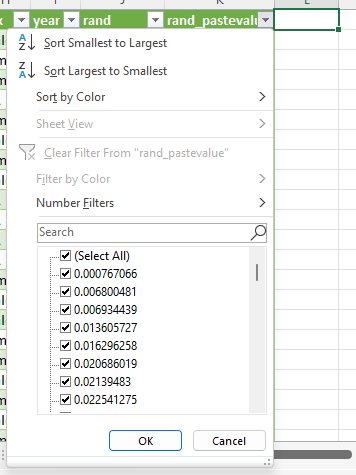
\includegraphics{./step3-sort1.png}

}

\caption{Sortir, jika tabel}

\end{figure}

Jika belum berbentuk tabel, pilih \emph{sampling frame} yang ingin
disortir, lalu klik \emph{sort \& filter}.

\begin{figure}

{\centering 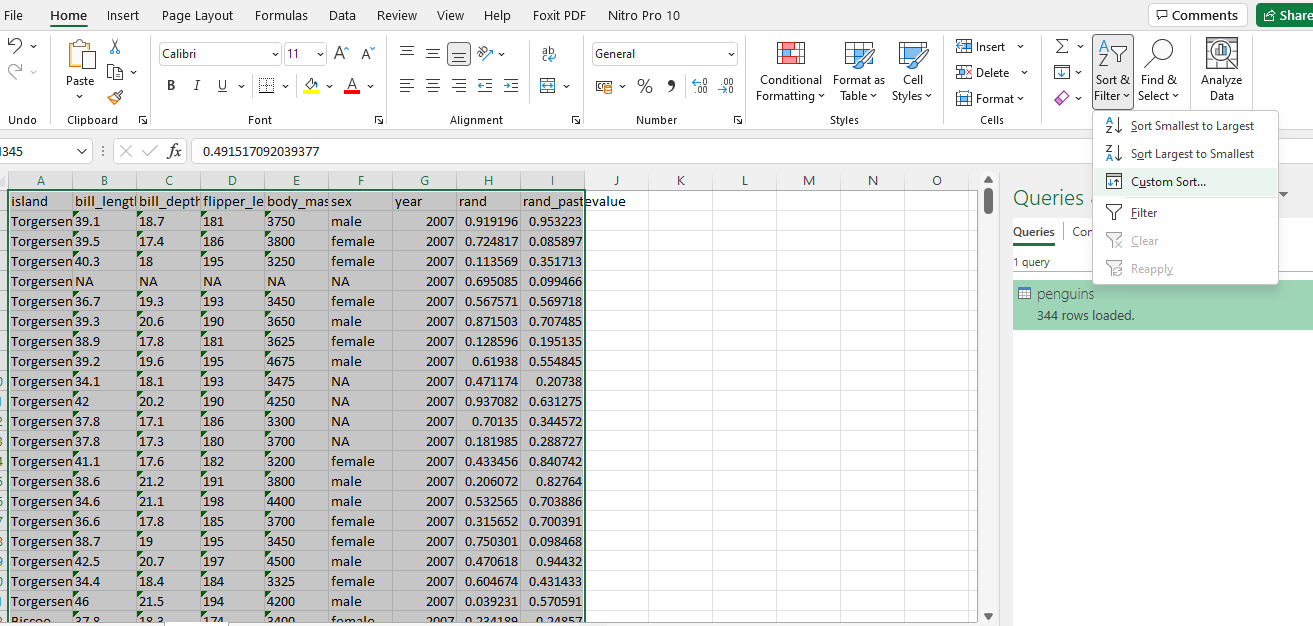
\includegraphics{./step-sort21.png}

}

\caption{Sortir, tanpa tabel}

\end{figure}

Lalu, pilih kolom nilai acak dan sortir.

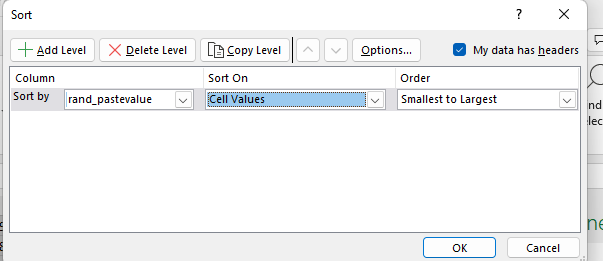
\includegraphics{./step2-sort22.png}

\hypertarget{r-3}{%
\subsubsection{R}\label{r-3}}

Sortir menggunakan \emph{arrange}.

\begin{Shaded}
\begin{Highlighting}[]
\NormalTok{penguins }\SpecialCharTok{|\textgreater{}} \FunctionTok{arrange}\NormalTok{(}\FunctionTok{desc}\NormalTok{(rando)) }\SpecialCharTok{|\textgreater{}}
  \FunctionTok{head}\NormalTok{(}\DecValTok{3}\NormalTok{) }\SpecialCharTok{|\textgreater{}}\NormalTok{ knitr}\SpecialCharTok{::}\FunctionTok{kable}\NormalTok{()}
\end{Highlighting}
\end{Shaded}

\begin{longtable}[]{@{}
  >{\raggedleft\arraybackslash}p{(\columnwidth - 18\tabcolsep) * \real{0.0577}}
  >{\raggedright\arraybackslash}p{(\columnwidth - 18\tabcolsep) * \real{0.0962}}
  >{\raggedright\arraybackslash}p{(\columnwidth - 18\tabcolsep) * \real{0.0673}}
  >{\raggedleft\arraybackslash}p{(\columnwidth - 18\tabcolsep) * \real{0.1442}}
  >{\raggedleft\arraybackslash}p{(\columnwidth - 18\tabcolsep) * \real{0.1346}}
  >{\raggedleft\arraybackslash}p{(\columnwidth - 18\tabcolsep) * \real{0.1731}}
  >{\raggedleft\arraybackslash}p{(\columnwidth - 18\tabcolsep) * \real{0.1154}}
  >{\raggedright\arraybackslash}p{(\columnwidth - 18\tabcolsep) * \real{0.0673}}
  >{\raggedleft\arraybackslash}p{(\columnwidth - 18\tabcolsep) * \real{0.0481}}
  >{\raggedleft\arraybackslash}p{(\columnwidth - 18\tabcolsep) * \real{0.0962}}@{}}
\toprule()
\begin{minipage}[b]{\linewidth}\raggedleft
rowid
\end{minipage} & \begin{minipage}[b]{\linewidth}\raggedright
species
\end{minipage} & \begin{minipage}[b]{\linewidth}\raggedright
island
\end{minipage} & \begin{minipage}[b]{\linewidth}\raggedleft
bill\_length\_mm
\end{minipage} & \begin{minipage}[b]{\linewidth}\raggedleft
bill\_depth\_mm
\end{minipage} & \begin{minipage}[b]{\linewidth}\raggedleft
flipper\_length\_mm
\end{minipage} & \begin{minipage}[b]{\linewidth}\raggedleft
body\_mass\_g
\end{minipage} & \begin{minipage}[b]{\linewidth}\raggedright
sex
\end{minipage} & \begin{minipage}[b]{\linewidth}\raggedleft
year
\end{minipage} & \begin{minipage}[b]{\linewidth}\raggedleft
rando
\end{minipage} \\
\midrule()
\endhead
93 & Adelie & Dream & 34.0 & 17.1 & 185 & 3400 & female & 2008 &
0.9931674 \\
283 & Chinstrap & Dream & 46.1 & 18.2 & 178 & 3250 & female & 2007 &
0.9877717 \\
321 & Chinstrap & Dream & 50.9 & 17.9 & 196 & 3675 & female & 2009 &
0.9871470 \\
\bottomrule()
\end{longtable}

\hypertarget{python-3}{%
\subsubsection{Python}\label{python-3}}

Gunakan
\texttt{namaDataset.sort\_values(by\ =\ "kolom\ angka\ acak",\ ...)}

\begin{Shaded}
\begin{Highlighting}[]
\ImportTok{import}\NormalTok{ pandas }\ImportTok{as}\NormalTok{ pd}

\NormalTok{penguins\_sorted }\OperatorTok{=}\NormalTok{ penguins.sort\_values(by }\OperatorTok{=} \StringTok{"randomNumber"}\NormalTok{, ascending}\OperatorTok{=}\VariableTok{False}\NormalTok{)}
\BuiltInTok{print}\NormalTok{(penguins\_sorted.head(}\DecValTok{58}\NormalTok{))}
\end{Highlighting}
\end{Shaded}

\begin{verbatim}
     randomNumber  rowid    species  ... body_mass_g     sex  year
82       0.998006     83     Adelie  ...      3800.0  female  2008
2        0.988113      3     Adelie  ...      3250.0  female  2007
179      0.985227    180     Gentoo  ...      5650.0    male  2007
64       0.982089     65     Adelie  ...      2850.0  female  2008
20       0.981606     21     Adelie  ...      3400.0  female  2007
316      0.979618    317  Chinstrap  ...      3950.0    male  2008
36       0.978045     37     Adelie  ...      3950.0    male  2007
226      0.971176    227     Gentoo  ...      4700.0  female  2008
88       0.968786     89     Adelie  ...      3950.0    male  2008
291      0.967539    292  Chinstrap  ...      4050.0    male  2007
142      0.964342    143     Adelie  ...      3050.0  female  2009
66       0.964280     67     Adelie  ...      3350.0  female  2008
192      0.964219    193     Gentoo  ...      3950.0  female  2008
245      0.962202    246     Gentoo  ...      5650.0    male  2009
337      0.957290    338  Chinstrap  ...      3650.0  female  2009
261      0.955021    262     Gentoo  ...      5500.0    male  2009
215      0.951514    216     Gentoo  ...      5650.0    male  2008
91       0.949608     92     Adelie  ...      4300.0    male  2008
73       0.949112     74     Adelie  ...      4150.0    male  2008
223      0.938686    224     Gentoo  ...      5000.0    male  2008
289      0.929323    290  Chinstrap  ...      4050.0    male  2007
242      0.923924    243     Gentoo  ...      4950.0  female  2009
317      0.914438    318  Chinstrap  ...      3650.0  female  2008
19       0.908108     20     Adelie  ...      4200.0    male  2007
197      0.906972    198     Gentoo  ...      4900.0  female  2008
177      0.905509    178     Gentoo  ...      5100.0    male  2007
229      0.901730    230     Gentoo  ...      6000.0    male  2008
54       0.900127     55     Adelie  ...      2900.0  female  2008
156      0.898963    157     Gentoo  ...      5400.0    male  2007
225      0.891437    226     Gentoo  ...      5200.0  female  2008
239      0.887460    240     Gentoo  ...      5300.0    male  2009
273      0.884751    274     Gentoo  ...      5750.0    male  2009
324      0.883531    325  Chinstrap  ...      3250.0    male  2009
23       0.881101     24     Adelie  ...      3950.0    male  2007
27       0.880034     28     Adelie  ...      3200.0  female  2007
175      0.876310    176     Gentoo  ...      5050.0    male  2007
134      0.876252    135     Adelie  ...      3425.0  female  2009
310      0.869858    311  Chinstrap  ...      3600.0    male  2008
272      0.866883    273     Gentoo  ...      4850.0  female  2009
106      0.861813    107     Adelie  ...      3750.0  female  2009
11       0.860677     12     Adelie  ...      3700.0     NaN  2007
280      0.857667    281  Chinstrap  ...      3725.0    male  2007
320      0.857076    321  Chinstrap  ...      3675.0  female  2009
70       0.855720     71     Adelie  ...      3600.0  female  2008
297      0.853891    298  Chinstrap  ...      3400.0    male  2007
189      0.849117    190     Gentoo  ...      5250.0    male  2008
110      0.832433    111     Adelie  ...      3825.0  female  2009
100      0.829604    101     Adelie  ...      3725.0  female  2009
178      0.828691    179     Gentoo  ...      4100.0     NaN  2007
234      0.828592    235     Gentoo  ...      4725.0  female  2009
194      0.824546    195     Gentoo  ...      4300.0  female  2008
195      0.821451    196     Gentoo  ...      4750.0    male  2008
202      0.819321    203     Gentoo  ...      4850.0  female  2008
247      0.818314    248     Gentoo  ...      5200.0    male  2009
307      0.817592    308  Chinstrap  ...      4300.0    male  2008
224      0.814083    225     Gentoo  ...      5100.0    male  2008
308      0.813684    309  Chinstrap  ...      3350.0  female  2008
257      0.807059    258     Gentoo  ...      5500.0    male  2009

[58 rows x 10 columns]
\end{verbatim}

\hypertarget{alternatif}{%
\subsection{Alternatif}\label{alternatif}}

\begin{enumerate}
\def\labelenumi{\arabic{enumi}.}
\tightlist
\item
  Buat \(n\) integer random dari \(1\) ke \(N\), jumlah populasi.
\item
  Ambil row yang sesuai integer random tersebut.
\end{enumerate}

\hypertarget{r-4}{%
\subsubsection{R}\label{r-4}}

\begin{Shaded}
\begin{Highlighting}[]
\FunctionTok{library}\NormalTok{(dplyr)}

\NormalTok{indexes }\OtherTok{\textless{}{-}} \FunctionTok{sample.int}\NormalTok{(}\AttributeTok{n =} \FunctionTok{nrow}\NormalTok{(penguins), }\AttributeTok{size =} \DecValTok{3}\NormalTok{)}
\NormalTok{penguins }\SpecialCharTok{|\textgreater{}} \FunctionTok{filter}\NormalTok{(rowid }\SpecialCharTok{\%in\%}\NormalTok{ indexes) }\SpecialCharTok{|\textgreater{}}\NormalTok{ knitr}\SpecialCharTok{::}\FunctionTok{kable}\NormalTok{()}
\end{Highlighting}
\end{Shaded}

\begin{longtable}[]{@{}
  >{\raggedleft\arraybackslash}p{(\columnwidth - 18\tabcolsep) * \real{0.0561}}
  >{\raggedright\arraybackslash}p{(\columnwidth - 18\tabcolsep) * \real{0.0935}}
  >{\raggedright\arraybackslash}p{(\columnwidth - 18\tabcolsep) * \real{0.0935}}
  >{\raggedleft\arraybackslash}p{(\columnwidth - 18\tabcolsep) * \real{0.1402}}
  >{\raggedleft\arraybackslash}p{(\columnwidth - 18\tabcolsep) * \real{0.1308}}
  >{\raggedleft\arraybackslash}p{(\columnwidth - 18\tabcolsep) * \real{0.1682}}
  >{\raggedleft\arraybackslash}p{(\columnwidth - 18\tabcolsep) * \real{0.1121}}
  >{\raggedright\arraybackslash}p{(\columnwidth - 18\tabcolsep) * \real{0.0654}}
  >{\raggedleft\arraybackslash}p{(\columnwidth - 18\tabcolsep) * \real{0.0467}}
  >{\raggedleft\arraybackslash}p{(\columnwidth - 18\tabcolsep) * \real{0.0935}}@{}}
\toprule()
\begin{minipage}[b]{\linewidth}\raggedleft
rowid
\end{minipage} & \begin{minipage}[b]{\linewidth}\raggedright
species
\end{minipage} & \begin{minipage}[b]{\linewidth}\raggedright
island
\end{minipage} & \begin{minipage}[b]{\linewidth}\raggedleft
bill\_length\_mm
\end{minipage} & \begin{minipage}[b]{\linewidth}\raggedleft
bill\_depth\_mm
\end{minipage} & \begin{minipage}[b]{\linewidth}\raggedleft
flipper\_length\_mm
\end{minipage} & \begin{minipage}[b]{\linewidth}\raggedleft
body\_mass\_g
\end{minipage} & \begin{minipage}[b]{\linewidth}\raggedright
sex
\end{minipage} & \begin{minipage}[b]{\linewidth}\raggedleft
year
\end{minipage} & \begin{minipage}[b]{\linewidth}\raggedleft
rando
\end{minipage} \\
\midrule()
\endhead
118 & Adelie & Torgersen & 37.3 & 20.5 & 199 & 3775 & male & 2009 &
0.9851804 \\
124 & Adelie & Torgersen & 41.4 & 18.5 & 202 & 3875 & male & 2009 &
0.0680086 \\
289 & Chinstrap & Dream & 47.0 & 17.3 & 185 & 3700 & female & 2007 &
0.6058434 \\
\bottomrule()
\end{longtable}

\hypertarget{python-4}{%
\subsubsection{Python}\label{python-4}}

\begin{Shaded}
\begin{Highlighting}[]
\ImportTok{import}\NormalTok{ pandas }\ImportTok{as}\NormalTok{ pd}
\ImportTok{import}\NormalTok{ numpy }\ImportTok{as}\NormalTok{ np}

\NormalTok{indexes }\OperatorTok{=}\NormalTok{ np.random.randint(}\DecValTok{0}\NormalTok{, }\BuiltInTok{len}\NormalTok{(penguins.index),}\DecValTok{5}\NormalTok{)}

\NormalTok{newpenguins }\OperatorTok{=}\NormalTok{ penguins[(penguins.index).isin(indexes)]}
\NormalTok{newpenguins}
\end{Highlighting}
\end{Shaded}

\begin{verbatim}
     randomNumber  rowid    species  ... body_mass_g     sex  year
49       0.337298     50     Adelie  ...      4150.0    male  2007
78       0.412398     79     Adelie  ...      3550.0  female  2008
106      0.861813    107     Adelie  ...      3750.0  female  2009
250      0.014140    251     Gentoo  ...      4625.0  female  2009
317      0.914438    318  Chinstrap  ...      3650.0  female  2008

[5 rows x 10 columns]
\end{verbatim}

\hypertarget{exercise-2}{%
\subsection{Exercise}\label{exercise-2}}

Bagi jadi 3 - ambil sampel sebanyak:

\begin{enumerate}
\def\labelenumi{\arabic{enumi}.}
\tightlist
\item
  40 dari dataset Iris
  (https://www.kaggle.com/datasets/arshid/iris-flower-dataset)
\item
  14 dari dataset mtcars
  (https://gist.github.com/seankross/a412dfbd88b3db70b74b)
\item
  58 dari dataset penguins
  (https://gist.github.com/slopp/ce3b90b9168f2f921784de84fa445651)
\end{enumerate}

\hypertarget{menduga-parameter-populasi}{%
\section{Menduga Parameter populasi}\label{menduga-parameter-populasi}}

Beberapa rumus yang digunakan untuk menduga parameter populasi:

\hypertarget{mean}{%
\subsubsection{Mean}\label{mean}}

\[
\begin{aligned}
\hat{\mu}&=\bar{y}=\frac{\sum_{i=1}^n y_i}{n} & \text{(mean)}\\
\hat{V}(\bar{y})&=\left(1-\frac{n}{N}\right)\frac{s^2}{n}&\text{(ragam penduga)}\\\
s^2&=\frac{1}{n-1}\sum_{i=1}^n(y_i-\bar{y})^2 &\\
\hat{\mu}&\pm2\sqrt{\hat{V}(\bar{y})} & \text{(selang kepercayaan)}
\end{aligned}
\]

Penduga bagi mean adalah rataan sampel, yaitu total nilai dari sampel
dibagi ukuran sampel. Bagaimana untuk ragam penduga? Penurunan rumus ini
dimulai dari nilai \(V\left(\bar{y}\right)\). Dalam kasus populasi tak
hingga yang saling bebas dan memiliki ragam sama:

\[
\begin{aligned}
V\left(\bar{y}\right)&=V\left(\frac{y_1+\ldots+y_n}{n}\right)=\frac{1}{n^2}V(y_1+\ldots+y_n)\\ 
&=\frac{V(y_1)+\ldots+V(y_n)}{n^2}=\frac{n\sigma}{n^2}=\frac{\sigma}{n}
\end{aligned}
\]

Jadi, misal ada 100 elemen yang diobservasi di sampel, ragam dari
rata-ratanya seharusnya menjadi \(\sigma/n\). Namun jika sampel
terhingga, misal 100, maka ragamnya bukan \(\sigma/n\). Harusnya nol
karena kita mengobservasi seluruh populasi!

Dengan logika yang sama, dalam kasus populasi terhingga, ukuran sampel
dianggap besar atau kecil relatif terhadap ukuran populasi. Jika
sebagian besar populasi sudah diambil di sampel walaupun \(n\) atau
ukuran absolutnya kecil, seharusnya ragam dari rata-rata berkurang
signifikan. Oleh karena itu, perlu ada \emph{faktor koreksi populasi
terhingga}. Dengan faktor koreksi tersebut, ditemukan bahwa

\[
\mathrm{Var}(\bar{y}) = \frac{\sigma^2}{n} \left( \frac{N-n}{N-1} \right)
\]

Untuk lengkapnya, baca di
\href{https://stats.stackexchange.com/questions/5158/explanation-of-finite-population-correction-factor}{sini}.

Lalu ternyata \(E(s^2)=\frac{N}{N-1}\sigma^2\). Derivasi ada di halaman
akhir buku Schaeffer. Oleh karena itu, agar pendugaan tak bias, perlu
dikalikan dengan \(\frac{N-n}{N}=\left(1-\frac{n}{N})\right\).

Selang kepercayaan \(95\%\) selalu akan memiliki bentuk
\$\hat{\mu}\&\pm2\sqrt{\hat{V}(\bar{y})} \$. Agar kepercayaan \(95\%\),
maka probabilitas di sisi kiri dan kanan masing masing \(2.5\%\).
\(Z_{0.025}=1.96\).

\hypertarget{total}{%
\subsubsection{Total}\label{total}}

\[
\begin{aligned}
\hat{\tau}&=N\bar{y}=\frac{N\sum_{i=1}^n y_i}{n} & \text{(total)}\\
\hat{V}(\hat{\tau})&=\hat{V}(N\bar{y})=N^2\left(1-\frac{n}{N}\right)\frac{s^2}{n}&\text{(ragam penduga)}\\\
\hat{\tau}&\pm2\sqrt{\hat{V}(\tau)} & \text{(selang kepercayaan)}
\end{aligned}
\]

Logika dari penduga ini adalah perkalian penduga-penduga mean sebelumnya
dengan ukuran populasi \(N\). Karena ragam merupakan semua bentuk
kuadrat, maka ukuran populasi dikuadratkan (\(N^2\)).

\hypertarget{proporsi}{%
\subsubsection{Proporsi}\label{proporsi}}

\[
\begin{aligned}
\hat{p}&=\bar{y}=\frac{\sum_{i=1}^n y_i}{n} & \text{(proporsi, y=1 atau 0)}\\
\hat{V}(\hat{p})&=\left(1-\frac{n}{N}\right)\frac{\hat{p}\hat{q}}{n-1}&\text{(ragam penduga)}\\
\hat{q}&=1-\hat{p}\\
\hat{p}&\pm2\sqrt{\hat{V}(p)} & \text{(selang kepercayaan)}
\end{aligned}
\]

Penduga ragam proporsi tersebut berasal dari sebaran Bernoulli. Peluang
satu observasi \(Y\) memiliki nilai 1 (sukses) atau 0 (gagal) dimodelkan
dengan:

\[
f(y)=p^{y}(1-p)^{1-y}
\]

Nilai harapannya adalah:

\[
0\cdot f(0)+1\cdot f(1)=p
\]

Dan ragamnya adalah:

\[
\begin{aligned}
(0-p)^2 f(o)+(1-p)^2f(1)&=p^2(1-p)+p(1-p)^2\\ 
&=p(p-p^2+1-2p+p^2)=p(1-p)\\ 
&=pq
\end{aligned}
\]

Yang menggantikan \(\sigma\) untuk satu observasi. Selebihnya, filosofi
penurunannya sama.

\hypertarget{cara-perhitungan-excel-cheatsheet}{%
\subsection{Cara Perhitungan: Excel
Cheatsheet}\label{cara-perhitungan-excel-cheatsheet}}

\hypertarget{mean-1}{%
\subsubsection{Mean}\label{mean-1}}

Asumsikan Anda ingin menghitung rata-rata \emph{bill length} dari 50
penguin di sebuah sampel dataset penguins. Asumsikan bahwa data tersebut
dikumpulkan melalui \emph{simple ranom sampling}, dari populasi 344
penguin di dataset.

\begin{figure}

{\centering 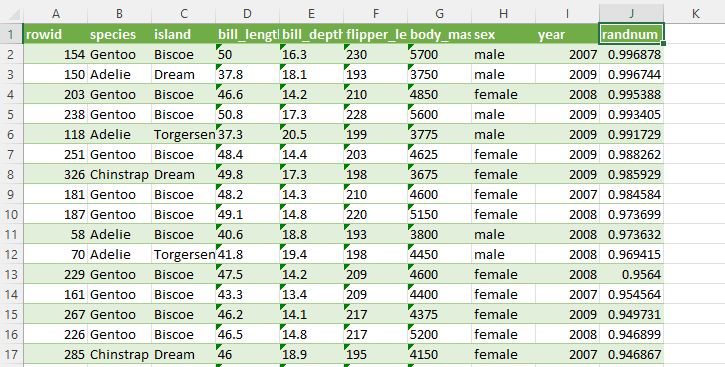
\includegraphics{./count-1.png}

}

\caption{Dataset}

\end{figure}

Sebelum menghitung rata-rata, perhatikan bahwa angka-angka di dataset
rata kiri. Ternyata, angka tersebut belum dianggap data numerik oleh
Excel. Oleh karena itu, buat kolom baru untuk konversi menggunakan
fungsi \texttt{VALUE}. Untuk baris pertama, misal, nilai \emph{bill
length} berada di D2. Oleh karena itu, nilai kolom baru tersebut adalah
\texttt{VALUE(D2)}.

\begin{figure}

{\centering 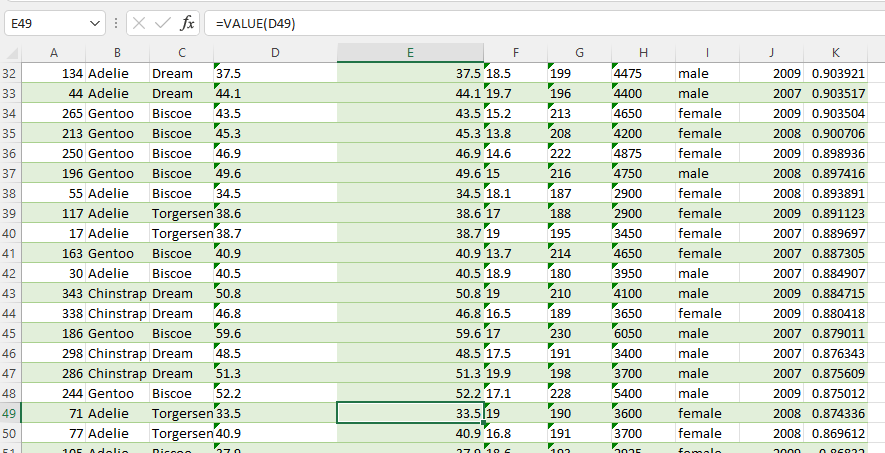
\includegraphics{./count-2.png}

}

\caption{Konversi}

\end{figure}

Langkah pertama adalah menghitung rata-rata. Bill length yang berbentuk
angka berada di kolom E, 2-51. Maka tuliskan \texttt{SUM(E2:E51)/50}
atau \texttt{AVERAGE(E2:E51)}

\begin{figure}

{\centering 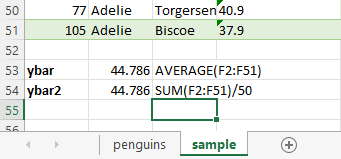
\includegraphics{./count-3.png}

}

\caption{Penduga rataan}

\end{figure}

Dapat dilakukan dua cara untuk menghitung simpangan baku sampel.
Pertama, dapat dibuat kolom simpangan \(y-\bar{y}\), lalu dikuadratkan.
Karena kita ingin mengurangi seluruh kolom E dengan konstanta di B53,
maka gunakan \texttt{\$B\$53} agar posisi sel yang mengandung rataan
sampel tidak berubah. \texttt{\$B} menetapkan indeks kolom (tidak
berubah jika di-\emph{copy} ke kanan-kiri) dan \texttt{\$53} menetapkan
indeks baris (tidak berubah jika di-\emph{copy} ke atas-bawah). Kolom E
tidak perlu diberi tanda \texttt{\$}. Justru, jika diberi tanda dolar di
\texttt{E\$1}, misal, indeks baris (angka) akan tetap di E1 walaupun
rumus di-\emph{copy} ke baris di bawahnya.

\begin{figure}

{\centering 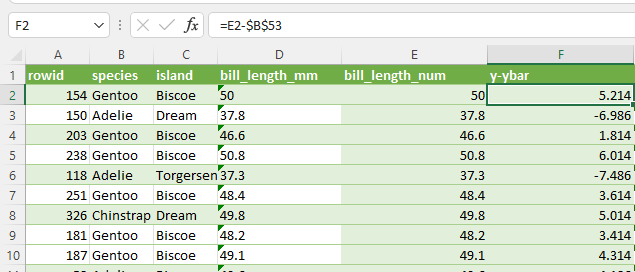
\includegraphics{./count-4.png}

}

\caption{Deviasi}

\end{figure}

Untuk mengkuadratkan, gunakan \texttt{{[}tempat\ sel{]}\^{}2}. Misal
ingin mengkuadratkan sel E1, maka tulis \texttt{E1\^{}2}. Gunakan
\texttt{SUM} untuk mencari jumlah, dan bagi \(n-1\). Atau, dapat
digunakan \texttt{VAR.S(RANGE)}. Jadi, buat \texttt{VAR.S(E2:E51)}.

\begin{figure}

{\centering 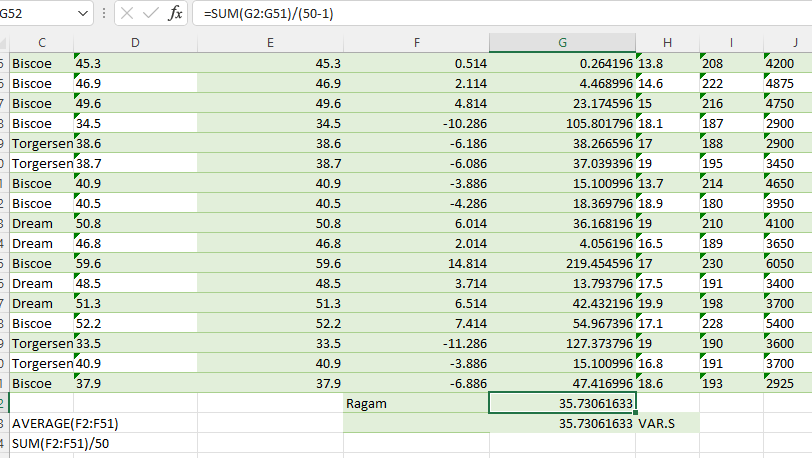
\includegraphics{./count-6.png}

}

\caption{Ragam}

\end{figure}

Lalu, hitung faktor koreksi dan \(1/n\). Gunakan \texttt{PRODUCT} untuk
menghitung perkalian:

\begin{figure}

{\centering 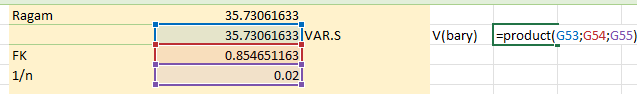
\includegraphics{./count-7.png}

}

\caption{Ragam penduga}

\end{figure}

BoE selalu memiliki bentuk \(2\sqrt{V(\hat{\mu})}\) untuk mean:

\begin{figure}

{\centering 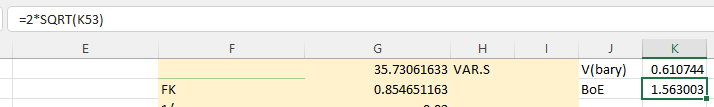
\includegraphics{./count-8.png}

}

\caption{BoE}

\end{figure}

\hypertarget{total-1}{%
\subsubsection{Total}\label{total-1}}

Karena diketahui bahwa:

\[
\hat{\tau}=N\bar{y};\quad \mathrm{V(\hat{\tau})}= \mathrm{V(N\bar{y})=N^2V(\bar{y})}
\]

Maka perhitungan cukup sederhana.

\begin{figure}

{\centering 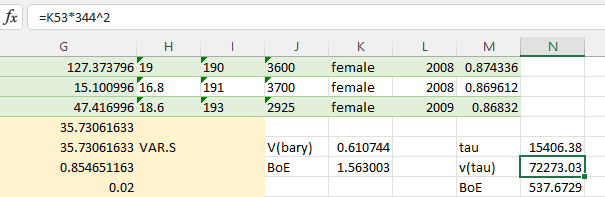
\includegraphics{./count-9.png}

}

\caption{Total}

\end{figure}

\hypertarget{proporsi-1}{%
\subsubsection{Proporsi}\label{proporsi-1}}

Misal ingin dihitung proporsi penguin laki-laki. Cara sederhana adalah
mengkonversi data kategorik jenis kelamin menjadi data biner 0/1
menggunakan fungsi \texttt{IF}. Misal jika baris pertama (K2) laki-laki,
buat menjadi 1. Jika tidak, buat menjadi 0. Jadi:
\texttt{IF(K2="male";\ 1;\ 0)}. Lalu tambahkan dan bagi 50 untuk
mendapat proporsi.

\begin{figure}

{\centering 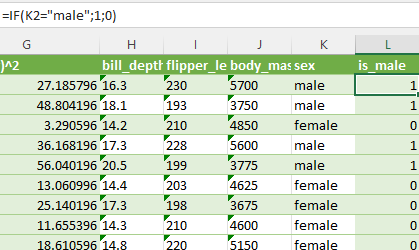
\includegraphics{./count-10.png}

}

\caption{Konversi}

\end{figure}

Sehingga hasilnya:

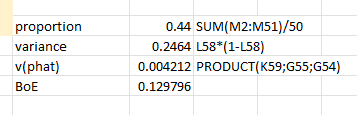
\includegraphics{./count-11.png}

\hypertarget{reporting-menggunakan-latex}{%
\subsection{Reporting menggunakan
LaTeX}\label{reporting-menggunakan-latex}}

Rumus-rumus matematika dapat ditulis dengan lebih mudah menggunakan
LaTeX. LaTeX dapat digunakan di Microsoft Word di menu \emph{Equation}.
Menu tersebut diakses menggunakan \texttt{Alt\ +\ Tab}.

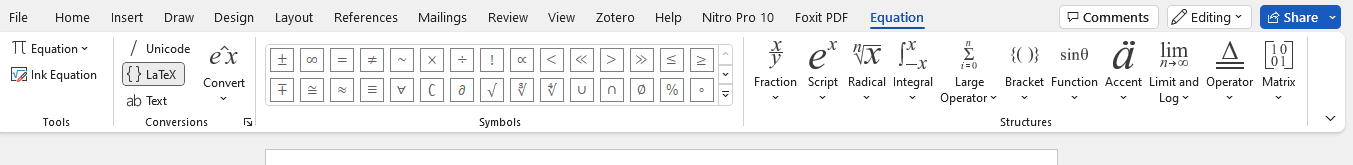
\includegraphics{./count-12.png}

Atau, dapat diakses menggunakan
\href{https://www.overleaf.com/}{Overleaf}.

Angka dituliskan di LaTeX seperti biasa. Simbol-simbol ditulis
menggunakan \texttt{\textbackslash{}namasimbol}, misal
\texttt{\textbackslash{}theta} untuk \(\theta\).
\texttt{\textbackslash{}mu} dan \texttt{\textbackslash{}sigma}
menuliskan \(\mu\) dan \(\sigma\). \texttt{\textbackslash{}bar\{y\}}
menghasilkan \(\bar{y}\) dan
\texttt{\textbackslash{}hat\{\textbackslash{}mu\}} menghasilkan
\(\hat{\mu}\).

Subskrip dan superskrip ditulis menggunakan \_ dan \^{}. Misal,
\texttt{y\_\{i3\}\^{}\{e4\}} menghasilkan \(y_{i3}^{e4}\). Pertambahan
ditulis menggunakan \texttt{\textbackslash{}sum}.

Pecahan ditulis menggunakan \texttt{\textbackslash{}frac\{\}\{\}}. Misal
\texttt{\textbackslash{}frac\{1\}\{2\}} menghasilkan \(\frac{1}{2}\).
Pertambahan dituliskan menggunakan \texttt{\textbackslash{}sum} dan
perkalian dituliskan menggunakan \texttt{\textbackslash{}prod}.

Ada beberapa \emph{environment} di LaTeX. \emph{Environment} yang cukup
penting adalah \emph{aligned}. Tiap baris dipisahkan menggunakan
\texttt{//}. Kesejajaran tiap baris dipastikan dengan tanda \texttt{\&}.
Misal \texttt{\&=} memastikan tanda sama dengan pertama di tiap baris
sejajar.

Misal, kode LaTeX untuk menuliskan penduga mean:

\begin{verbatim}
\begin{aligned}
\hat{\mu}&=\bar{y}=\frac{\sum_{i=1}^n y_i}{n} & \text{(mean)}\\
\hat{V}(\bar{y})&=\left(1-\frac{n}{N}\right)\frac{s^2}{n}&\text{(ragam penduga)}\\\
s^2&=\frac{1}{n-1}\sum_{i=1}^n(y_i-\bar{y})^2 &\\
\hat{\mu}&\pm2\sqrt{\hat{V}(\bar{y})} & \text{(selang kepercayaan)}
\end{aligned}
\end{verbatim}

\hypertarget{exercise-3}{%
\subsection{Exercise}\label{exercise-3}}

Hitung mean, total, dan proporsi 3 variabel di sampel yang kamu ambil.
Bandingkan dengan nilai parameter populasi:

\begin{enumerate}
\def\labelenumi{\arabic{enumi}.}
\tightlist
\item
  Apakah sama?
\item
  Apakah nilai parameter populasi masuk selang kepercayaan?
\end{enumerate}

\hypertarget{menghitung-ukuran-sampel}{%
\section{Menghitung Ukuran Sampel}\label{menghitung-ukuran-sampel}}

Penduga untuk ukuran sampel secara umum ditemukan dengan memodifikasi
rumus BoE. Ingat bahwa BoE adalah \(2\sqrt{V(\bar{y})}\). Oleh karena
itu, ukuran sampel yang mengontrol BoE menjadi jumlah tertentu ditemukan
dengan memanipulasi rumus tersebut.

\hypertarget{mean-2}{%
\subsubsection{Mean}\label{mean-2}}

\[
\begin{aligned}
n=\frac{N\sigma^2}{(N-1)D+\sigma^2}; \quad D=\frac{B^2}{4}
\end{aligned}
\]

Rumus itu tidak lain ditemukan dari:

\[
\begin{aligned}
\mathrm{Var}(\bar{y})&= \frac{\sigma^2}{n} \left( \frac{N-n}{N-1} \right)\\ 
B&=2\sqrt{\mathrm{V}(\bar{y})}\\ 
\sqrt{D}&=\frac{B}{2}=\sqrt{\frac{\sigma^2}{n} \left( \frac{N-n}{N-1} \right)}\\ 
D&=\frac{\sigma^2}{n} \left( \frac{N-n}{N-1} \right)=\frac{1}{n}\left(\frac{\sigma^2N-\sigma^2n}{N-1}\right)\\ 
n&=\frac{\sigma^2N-\sigma^2n}{ND-D}\\ 
n+\frac{\sigma^2n}{ND-D}&=\frac{\sigma^2N}{ND-D}\\ 
n\left(1+\frac{\sigma^2}{ND-D}\right)&=\frac{\sigma^2N}{ND-D}\\ 
n&=\frac{\sigma^2N}{ND-D}\cdot\frac{ND-D}{ND-D+\sigma^2}=\frac{N\sigma^2}{(N-1)D+\sigma^2}
\end{aligned}
\]

Penurunan untuk kasus-kasus lain akan relatif sama dengan penurunan ini.

\hypertarget{total-2}{%
\subsubsection{Total}\label{total-2}}

\[
\begin{aligned}
n=\frac{N\sigma^2}{(N-1)D+\sigma^2}; \quad D=\frac{B^2}{4N^2}
\end{aligned}
\]

Rumus ini ditemukan dari fakta bahwa \(\tau=N\bar{y}\) sehingga:

\[
\begin{aligned}
B&=2\sqrt{\mathrm{V}(N\bar{y})}=2\sqrt{N^2 V(\bar{y})}=2N\sqrt{V(\bar{y})}\\ 
\sqrt{D}&=\frac{B}{2N}=\sqrt{V(\bar{y})}\\ 
\end{aligned}
\]

Yang diturunkan dengan cara sama seperti sebelumnya.

\hypertarget{proporsi-2}{%
\subsubsection{Proporsi}\label{proporsi-2}}

\[
\begin{aligned}
n=\frac{Npq}{(N-1)D+pq}; \quad D=\frac{B^2}{4N}, \ q=1-p
\end{aligned}
\]

\(\sigma^2\) digantikan saja dengan \(pq\), dengan alasan yang
dijelaskan di penduga ragam proporsi.

Keuntungan perhitungan ukuran sampel untuk proporsi adalah dapat
dihitung jika \(p\) dan \(q\) tidak diketahui. Dapat diasumsikan \(p\)
dan \(q\) yang memaksimumkan ragam, yaitu \(0.5\) (ambil turunan pertama
dari \(p-p^2\)).

\hypertarget{membandingkan-penduga}{%
\section{Membandingkan Penduga}\label{membandingkan-penduga}}

Untuk dua peubah acak \(y_1\) dan \(y_2\):

\[
E(y_1-y_2)=E(y_1)-E(y_2)
\]

Dan:

\[
V(y_1-y_2)=V(y_1)+V(y_2)-2\mathrm{Cov}(y_1,y_2)
\]

Jika \(y_1\) dan \(y_2\) saling bebas \(\mathrm{Cov}(y_1,y_2)=0\). Jika
\(y_1, \ldots, y_n\) dan \(x_1, \ldots, x_m\) saling bebas dengan
rata-rata \(\mu_x\) dan \(\mu_y\). Maka jika diduga menggunakan
\(\bar{y}-\bar{x}\).

\[
E(\bar{y}-\bar{x})=E(\bar{y})-E(\bar{x})=\mu_y-\mu_x
\]

Dan:

\[
V(\bar{y}-\bar{x})=V(\bar{y})+V(\bar{x})
\]

Yang ditemukan melalui rumus sebelumnya.

\bookmarksetup{startatroot}

\hypertarget{stratified-random-sampling}{%
\chapter{Stratified Random Sampling}\label{stratified-random-sampling}}

Tujuan dari sampling dalam survei adalah memaksimumkan informasi dengan
batasan biaya tertentu. Terkadang, lebih banyak informasi (atau BoE)
lebih rendah dapat ditemukan dengan menggunakan \textbf{stratified
random sampling}. Contoh acak berlapis diambil dengan memisahkan
populasi menjadi beberapa kelompok yang tidak tumpang tindih, disebut
\emph{strata}, dan mengambil contoh acak sederhana di tiap
\emph{strata}/lapisan.

Sebagai ilustrasi, sebuah survei hendak dilakukan untuk menduga warga
yang mendukung meningkatkan alokasi anggaran di suatu kabupaten untuk
memperbaiki layanan ambulans. Di kabupaten tersebut, terdapat dua area
perkotaan dan sebuah area desa. Dapat diambil contoh acak sederhana di
tiap kota dan di pedesaan. Dua kota dan satu desa menjadi tiga strata di
mana contoh acak sederhana diambil. Mengapa dipilih contoh acak
berlapis?

\begin{enumerate}
\def\labelenumi{\arabic{enumi}.}
\tightlist
\item
  Contoh acak yang memiliki keragaman kecil di antara elemennya akan
  menghasilkan BoE kecil. Jika warga tiap kota memiliki opini yang
  mirip, sampel di tiap strata akan memiliki keragaman kecil. Misal kota
  A memiliki rumah sakit sehingga ambulans tidak dibutuhkan. Namun, kota
  B tidak memiliki rumah sakit sehingga membutuhkan ambulans. Opini yang
  berbeda lagi dimiliki masyarakat desa yang mungkin jauh dari fasilitas
  tertentu.
\item
  Jika lapisan diatur sedemikian rupa sehingga surveyor lebih mudah
  memilih responden dan melaksanakan survei di area geografis yang
  dekat, biaya dapat dikurangi.
\item
  Dapat melakukan pendugaan parameter untuk tiap lapisan. Misal,
  pemerintahan kota A ingin mengetahui opini masyarakat kota tersebut.
  Proporsi tersebut dapat dihitung.
\end{enumerate}

Oleh karena itu, contoh acak berlapis dapat dipilih karena:

\begin{enumerate}
\def\labelenumi{\arabic{enumi}.}
\tightlist
\item
  Stratifikasi dapat menghasilkan BoE lebih kecil daripada contoh acak
  sederhana. Ini terjadi jika elemen \textbf{di dalam strata homogen}
  dan \textbf{antarstrata homogen}
\item
  Harga pengamatan dapat dikurangi jika strata dikelompokkan sedemikian
  rupa sehingga memudahkan pengamatan.
\item
  Penduga parameter dapat ditemukan untuk tiap strata.
\end{enumerate}

\hypertarget{mengambil-contoh-acak-berlapis}{%
\section{Mengambil Contoh Acak
Berlapis}\label{mengambil-contoh-acak-berlapis}}

Langkah pertama dari mengambil contoh acak berlapis adalah
menspesifikasi strata dan memasukkan tiap unit percontohan ke strata
yang tepat. Setelah itu, ambil contoh acak sederhana di tiap strata.

\hypertarget{pendugaan-parameter}{%
\section{Pendugaan Parameter}\label{pendugaan-parameter}}

Penduga-penduga parameter di contoh acak berlapis adalah:

\hypertarget{mean-3}{%
\subsubsection{Mean}\label{mean-3}}

\[
\begin{aligned}
\hat{\mu}&=\bar{y}_{st}=\frac{1}{N}[N_1\bar{y}_1+N_2\bar{y}_2+\ldots+N_L\bar{y}_L]& \text{(mean)}\\
&=\frac{1}{N}\sum_{i=1}^L N_i\bar{y}_i\\
\hat{V}(\bar{y_{st}})&=\frac{1}{N^2}\left[N_1^2 V(\bar{y_1})+N_1^2 V(\bar{y_2})+\ldots+N_L^2 V(\bar{y_L})\right]\\
&=\frac{1}{N^2}\left[N_1^2\left(1-\frac{n_1}{N_1}\right)\frac{s_1^2}{n_1}+\ldots\right]\\
&=\frac{1}{N^2}\sum_{i=1}^L N_i^2\left(1-\frac{n_i}{N_i}\right)\frac{s_i^2}{n_i}&\text{(ragam penduga)}\\\
\hat{\mu}&\pm2\sqrt{\hat{V}(\bar{y})} & \text{(selang kepercayaan)}
\end{aligned}
\]

Bagaimana penduga tersebut diturunkan? Pertama, rata-rata dihitung di
tiap strata. Namun, tidak cukup untuk menghitung rata-rata dari
rata-rata. Tiap strata harusnya mendapat bobot yang berbeda karena
jumlah populasi di tiap strata berbeda juga. Strata yang berkontribusi
banyak ke populasi (dalam kata lain, menyusun sebagian besar dari
populasi) seharusnya memiliki bobot lebih besar daripada strata yang
berkontribusi sedikit. Oleh karena itu, tiap rataan strata diboboti
dengan jumlah elemen di tiap strata dalam populasi.

Atau, dapat diturunkan dengan menghitung total terlebih dahulu. Dugaan
total tidak lain adalah pertambahan dari dugaan total tiap strata, dan
dugaan total untuk strata ke-i adalah \(N_i\bar{y}_i\). Lalu, dugaan
total tersebut dibagi dengan ukuran populasi sehingga jadi rata-rata.
Oleh karena itu, rumus rata-rata tersebut ditemukan.

Karena rataan tiap strata dianggap saling bebas jika pengacakan benar,
ragam hanya perlu ditambahkan.

\hypertarget{total-3}{%
\subsubsection{Total}\label{total-3}}

\[
\begin{aligned}
\hat{\tau}&=N\bar{y}_{st}=N_1\bar{y}_1+N_2\bar{y}_2+\ldots+N_L\bar{y}_L&\\
&= \sum_{i=1}^L N_i\bar{y}_i &  \text{(total)}\\
\hat{V}(N\bar{y}_{st})&=N^2V(\bar{y}_{st})\\ 
&=\sum_{i=1}^L N_i^2\left(1-\frac{n_i}{N_i}\right)\frac{s_i^2}{n_i}&\text{(ragam penduga)}\\\
\hat{\tau}&\pm2\sqrt{\hat{V}(\bar{Ny_{st}})} & \text{(selang kepercayaan)}
\end{aligned}
\]

Penduga tersebut tidak lain penduga mean yang dikali \(N\) saja.

\hypertarget{proporsi-3}{%
\subsubsection{Proporsi}\label{proporsi-3}}

\[
\begin{aligned}
\hat{p_{st}}&=\frac{1}{N}[N_1\hat{p}_1+N_2\hat{p}_2+\ldots+N_L\hat{p}_L]& \text{(proporsi)}\\
&= \frac{1}{N}\sum_{i=1}^L N_i\hat{p}_i\\
\hat{V}(\bar{y_{st}})&=\frac{1}{N^2}\left[N_1^2 V(\hat{p}_1)+N_1^2 V(\hat{p}_2)+\ldots+N_L^2 V(\hat{p}_L)\right]\\
&=\frac{1}{N^2}\left[N_1^2\left(1-\frac{n_1}{N_1}\right)\frac{\hat{p_1}\hat{q_1}}{n_1}+\ldots\right]\\
 &=\frac{1}{N^2}\sum_{i=1}^L N_i^2\left(1-\frac{n_i}{N_i}\right)\frac{\hat{p_I}\hat{q_I}}{n_i}&\text{(ragam penduga)}\\\
\hat{p}&\pm2\sqrt{\hat{V}(\hat{p})} & \text{(selang kepercayaan)}
\end{aligned}
\]

Sama seperti mean, tapi \(s^2\) diduga dengan \(pq\).

\hypertarget{contoh-perhitungan}{%
\section{Contoh perhitungan}\label{contoh-perhitungan}}

Bayangkan survei yang dijelaskan di skenario sebelumnya benar dilakukan.
Dalam kata lain, dilakukan pengambilan contoh acak berlapis dari 2 kota
(A dan B) serta daerah pedesaan. Objek survei adalah rata-rata jam yang
dihabiskan per hari untuk menonton televisi. Lalu terkumpul data:

\begin{Shaded}
\begin{Highlighting}[]
\NormalTok{townrural }\OtherTok{\textless{}{-}} \FunctionTok{read.csv2}\NormalTok{(}\StringTok{"ocrdat1.csv"}\NormalTok{) }

\NormalTok{townrural }\SpecialCharTok{|\textgreater{}}\NormalTok{ knitr}\SpecialCharTok{::}\FunctionTok{kable}\NormalTok{()}
\end{Highlighting}
\end{Shaded}

\begin{longtable}[]{@{}llllll@{}}
\toprule()
Strata & N & n & Mean & Median & SD \\
\midrule()
\endhead
Town A & 155.00 & 20.00 & 33.90 & 34.50 & 5.95 \\
Town B & 62.00 & 8.00 & 25.12 & 26.00 & 15.25 \\
Rural & 93.00 & 12.00 & 19.00 & 17.50 & 9.36 \\
\bottomrule()
\end{longtable}

Lakukan pendugaan rataan dan BoE! Kasus ini akan diilustrasikan
menggunakan R. Pertama, untuk menduga rataan, hitung \(N_iy_i\) lalu
tambahkan. Buat peubah baru, yaitu \(N_iy_i\). Namun, ternyata semua
peubah masih karakter:

\begin{Shaded}
\begin{Highlighting}[]
\NormalTok{townrural }\SpecialCharTok{|\textgreater{}} \FunctionTok{summary}\NormalTok{()}
\end{Highlighting}
\end{Shaded}

\begin{verbatim}
    Strata               N                  n                 Mean          
 Length:3           Length:3           Length:3           Length:3          
 Class :character   Class :character   Class :character   Class :character  
 Mode  :character   Mode  :character   Mode  :character   Mode  :character  
    Median               SD           
 Length:3           Length:3          
 Class :character   Class :character  
 Mode  :character   Mode  :character  
\end{verbatim}

\texttt{dplyr::mutate(across)} dapat membantu. Fungsi ini membuat peubah
baru sesuai dengan fungsi yang diinginkan:

\begin{Shaded}
\begin{Highlighting}[]
\FunctionTok{library}\NormalTok{(dplyr)}
\end{Highlighting}
\end{Shaded}

\begin{verbatim}

Attaching package: 'dplyr'
\end{verbatim}

\begin{verbatim}
The following objects are masked from 'package:stats':

    filter, lag
\end{verbatim}

\begin{verbatim}
The following objects are masked from 'package:base':

    intersect, setdiff, setequal, union
\end{verbatim}

\begin{Shaded}
\begin{Highlighting}[]
\NormalTok{townrural }\SpecialCharTok{|\textgreater{}} \FunctionTok{mutate}\NormalTok{(}\FunctionTok{across}\NormalTok{(}\SpecialCharTok{!}\NormalTok{Strata, as.numeric)) }\SpecialCharTok{|\textgreater{}} \FunctionTok{summary}\NormalTok{()}
\end{Highlighting}
\end{Shaded}

\begin{verbatim}
    Strata                N               n              Mean      
 Length:3           Min.   : 62.0   Min.   : 8.00   Min.   :19.00  
 Class :character   1st Qu.: 77.5   1st Qu.:10.00   1st Qu.:22.06  
 Mode  :character   Median : 93.0   Median :12.00   Median :25.12  
                    Mean   :103.3   Mean   :13.33   Mean   :26.01  
                    3rd Qu.:124.0   3rd Qu.:16.00   3rd Qu.:29.51  
                    Max.   :155.0   Max.   :20.00   Max.   :33.90  
     Median            SD        
 Min.   :17.50   Min.   : 5.950  
 1st Qu.:21.75   1st Qu.: 7.655  
 Median :26.00   Median : 9.360  
 Mean   :26.00   Mean   :10.187  
 3rd Qu.:30.25   3rd Qu.:12.305  
 Max.   :34.50   Max.   :15.250  
\end{verbatim}

Lalu buat peubah \(N_iy_i\). Lakukan \texttt{mutate}, dengan fungsi
\texttt{N*Mean}.

\begin{Shaded}
\begin{Highlighting}[]
\NormalTok{townrural }\SpecialCharTok{|\textgreater{}} 
    \FunctionTok{mutate}\NormalTok{(}\FunctionTok{across}\NormalTok{(}\SpecialCharTok{!}\NormalTok{Strata, as.numeric)) }\SpecialCharTok{|\textgreater{}}
    \FunctionTok{mutate}\NormalTok{(}\AttributeTok{Niybari =}\NormalTok{ N}\SpecialCharTok{*}\NormalTok{Mean) }\SpecialCharTok{|\textgreater{}}\NormalTok{ knitr}\SpecialCharTok{::}\FunctionTok{kable}\NormalTok{()}
\end{Highlighting}
\end{Shaded}

\begin{longtable}[]{@{}lrrrrrr@{}}
\toprule()
Strata & N & n & Mean & Median & SD & Niybari \\
\midrule()
\endhead
Town A & 155 & 20 & 33.90 & 34.5 & 5.95 & 5254.50 \\
Town B & 62 & 8 & 25.12 & 26.0 & 15.25 & 1557.44 \\
Rural & 93 & 12 & 19.00 & 17.5 & 9.36 & 1767.00 \\
\bottomrule()
\end{longtable}

Jumlahkan dan bagi:

\begin{Shaded}
\begin{Highlighting}[]
\NormalTok{townrural }\SpecialCharTok{|\textgreater{}} 
    \FunctionTok{mutate}\NormalTok{(}\FunctionTok{across}\NormalTok{(}\SpecialCharTok{!}\NormalTok{Strata, as.numeric)) }\SpecialCharTok{|\textgreater{}}
    \FunctionTok{mutate}\NormalTok{(}\AttributeTok{Niybari =}\NormalTok{ N}\SpecialCharTok{*}\NormalTok{Mean) }\SpecialCharTok{|\textgreater{}} 
    \FunctionTok{summarise}\NormalTok{(}\AttributeTok{ybar =} \FunctionTok{sum}\NormalTok{(Niybari)}\SpecialCharTok{/}\FunctionTok{sum}\NormalTok{(N))}
\end{Highlighting}
\end{Shaded}

\begin{verbatim}
    ybar
1 27.674
\end{verbatim}

Bagaimana dengan ragam? Sama saja, buat kolom \(N_i^2\), kolom faktor
koreksi, dan kolom \(s_i^2/n_i\). Gunakan \texttt{mutate} lagi, lalu
\texttt{summarize} untuk menyimpulkan:

\begin{Shaded}
\begin{Highlighting}[]
\NormalTok{townrural }\SpecialCharTok{|\textgreater{}} 
    \FunctionTok{mutate}\NormalTok{(}\FunctionTok{across}\NormalTok{(}\SpecialCharTok{!}\NormalTok{Strata, as.numeric)) }\SpecialCharTok{|\textgreater{}}
    \FunctionTok{mutate}\NormalTok{(}\AttributeTok{Nisq =}\NormalTok{ N}\SpecialCharTok{\^{}}\DecValTok{2}\NormalTok{,}
           \AttributeTok{FK =} \DecValTok{1}\SpecialCharTok{{-}}\NormalTok{n}\SpecialCharTok{/}\NormalTok{N,}
           \AttributeTok{sisqperni =}\NormalTok{ SD}\SpecialCharTok{\^{}}\DecValTok{2}\SpecialCharTok{/}\NormalTok{n) }\SpecialCharTok{|\textgreater{}}
    \FunctionTok{mutate}\NormalTok{(}\AttributeTok{varybar =}\NormalTok{ Nisq}\SpecialCharTok{*}\NormalTok{FK}\SpecialCharTok{*}\NormalTok{sisqperni) }\SpecialCharTok{|\textgreater{}}
    \FunctionTok{summarize}\NormalTok{(}\FunctionTok{sum}\NormalTok{(varybar)}\SpecialCharTok{/}\NormalTok{(}\FunctionTok{sum}\NormalTok{(N)}\SpecialCharTok{\^{}}\DecValTok{2}\NormalTok{))}
\end{Highlighting}
\end{Shaded}

\begin{verbatim}
  sum(varybar)/(sum(N)^2)
1                1.970491
\end{verbatim}



\end{document}
